% =========================================================================
% Supplementary Material -- "Source-Level Reliability Estimation"
% Companion to the ECIR 2027 "IR for Good" submission.
%
% IMPORTANT -- this is NOT part of the submitted PDF.
% ECIR 2027 makes no provision for supplementary material: the call mentions
% only appendices, and those "count toward the page limit" and must be placed
% "before the references". With the paper already over 12 pages, this document
% is meant to be hosted externally (OSF/Zenodo) and cited from the paper, which
% is what the rejected TCSS version did.
%
% Because the paper is under DOUBLE-BLIND review, anything linked from it must
% not identify the authors. Keep \anonymoustrue until acceptance; flip it for
% the camera-ready to restore the author block and the funding note.
%
% Build:  pdflatex supplementary && pdflatex supplementary
% =========================================================================
\documentclass[11pt,a4paper]{article}
\usepackage[margin=1in]{geometry}
\usepackage{graphicx,hyperref,amsmath,booktabs,subcaption}
\usepackage[numbers]{natbib}
\usepackage{orcidlink}
\usepackage{authblk}

\newif\ifanonymous
\anonymoustrue   % <-- comment out for the camera-ready

\title{Supplementary Material for\\
``Source-Level Reliability Estimation under Publisher-Disjoint Evaluation''}

\ifanonymous
  \author{}
  \date{}
\else
  \author[1]{John~Bianchi\,\orcidlink{0009-0006-2582-1480}\thanks{Corresponding author: john.bianchi@imtlucca.it}}
  \author[2]{Manuel~Pratelli\,\orcidlink{0000-0002-9978-791X}}
  \author[1]{Fabio~Pinelli\,\orcidlink{0000-0003-1058-6917}}
  \author[2,1]{Marinella~Petrocchi\,\orcidlink{0000-0003-0591-877X}}
  \affil[1]{IMT School for Advanced Studies Lucca, 55100 Lucca, Italy}
  \affil[2]{Institute of Informatics and Telematics, National Research Council (IIT-CNR), 56124 Pisa, Italy}
  \date{}
\fi

\renewcommand\Authands{ and }

\begin{document}
\maketitle

\ifanonymous
\else
  \footnotetext[1]{J. Bianchi: john.bianchi@imtlucca.it}
  \footnotetext[2]{M. Pratelli: manuel.pratelli@iit.cnr.it}
  \footnotetext[3]{F. Pinelli: fabio.pinelli@imtlucca.it}
  \footnotetext[4]{M. Petrocchi: marinella.petrocchi@iit.cnr.it}
  \footnotetext[5]{This work is partially supported by IIT-CNR internal project SIMULARE `SIMULAzione delle Reazioni alla disinformazionE con LLM'.}
\fi

\vspace{-1.5em}
\begin{center}
\textit{This supplementary material accompanies the main manuscript submitted to ECIR 2027, ``IR for Good'' track.}
\end{center}


\section{Model performance}
\label{app:performance_cms}
Figure \ref{fig:performance_cms} shows the confusion matrices for each fold and for the average.

\begin{figure*}[!t]
\centering
\begin{subfigure}[b]{0.48\linewidth}
  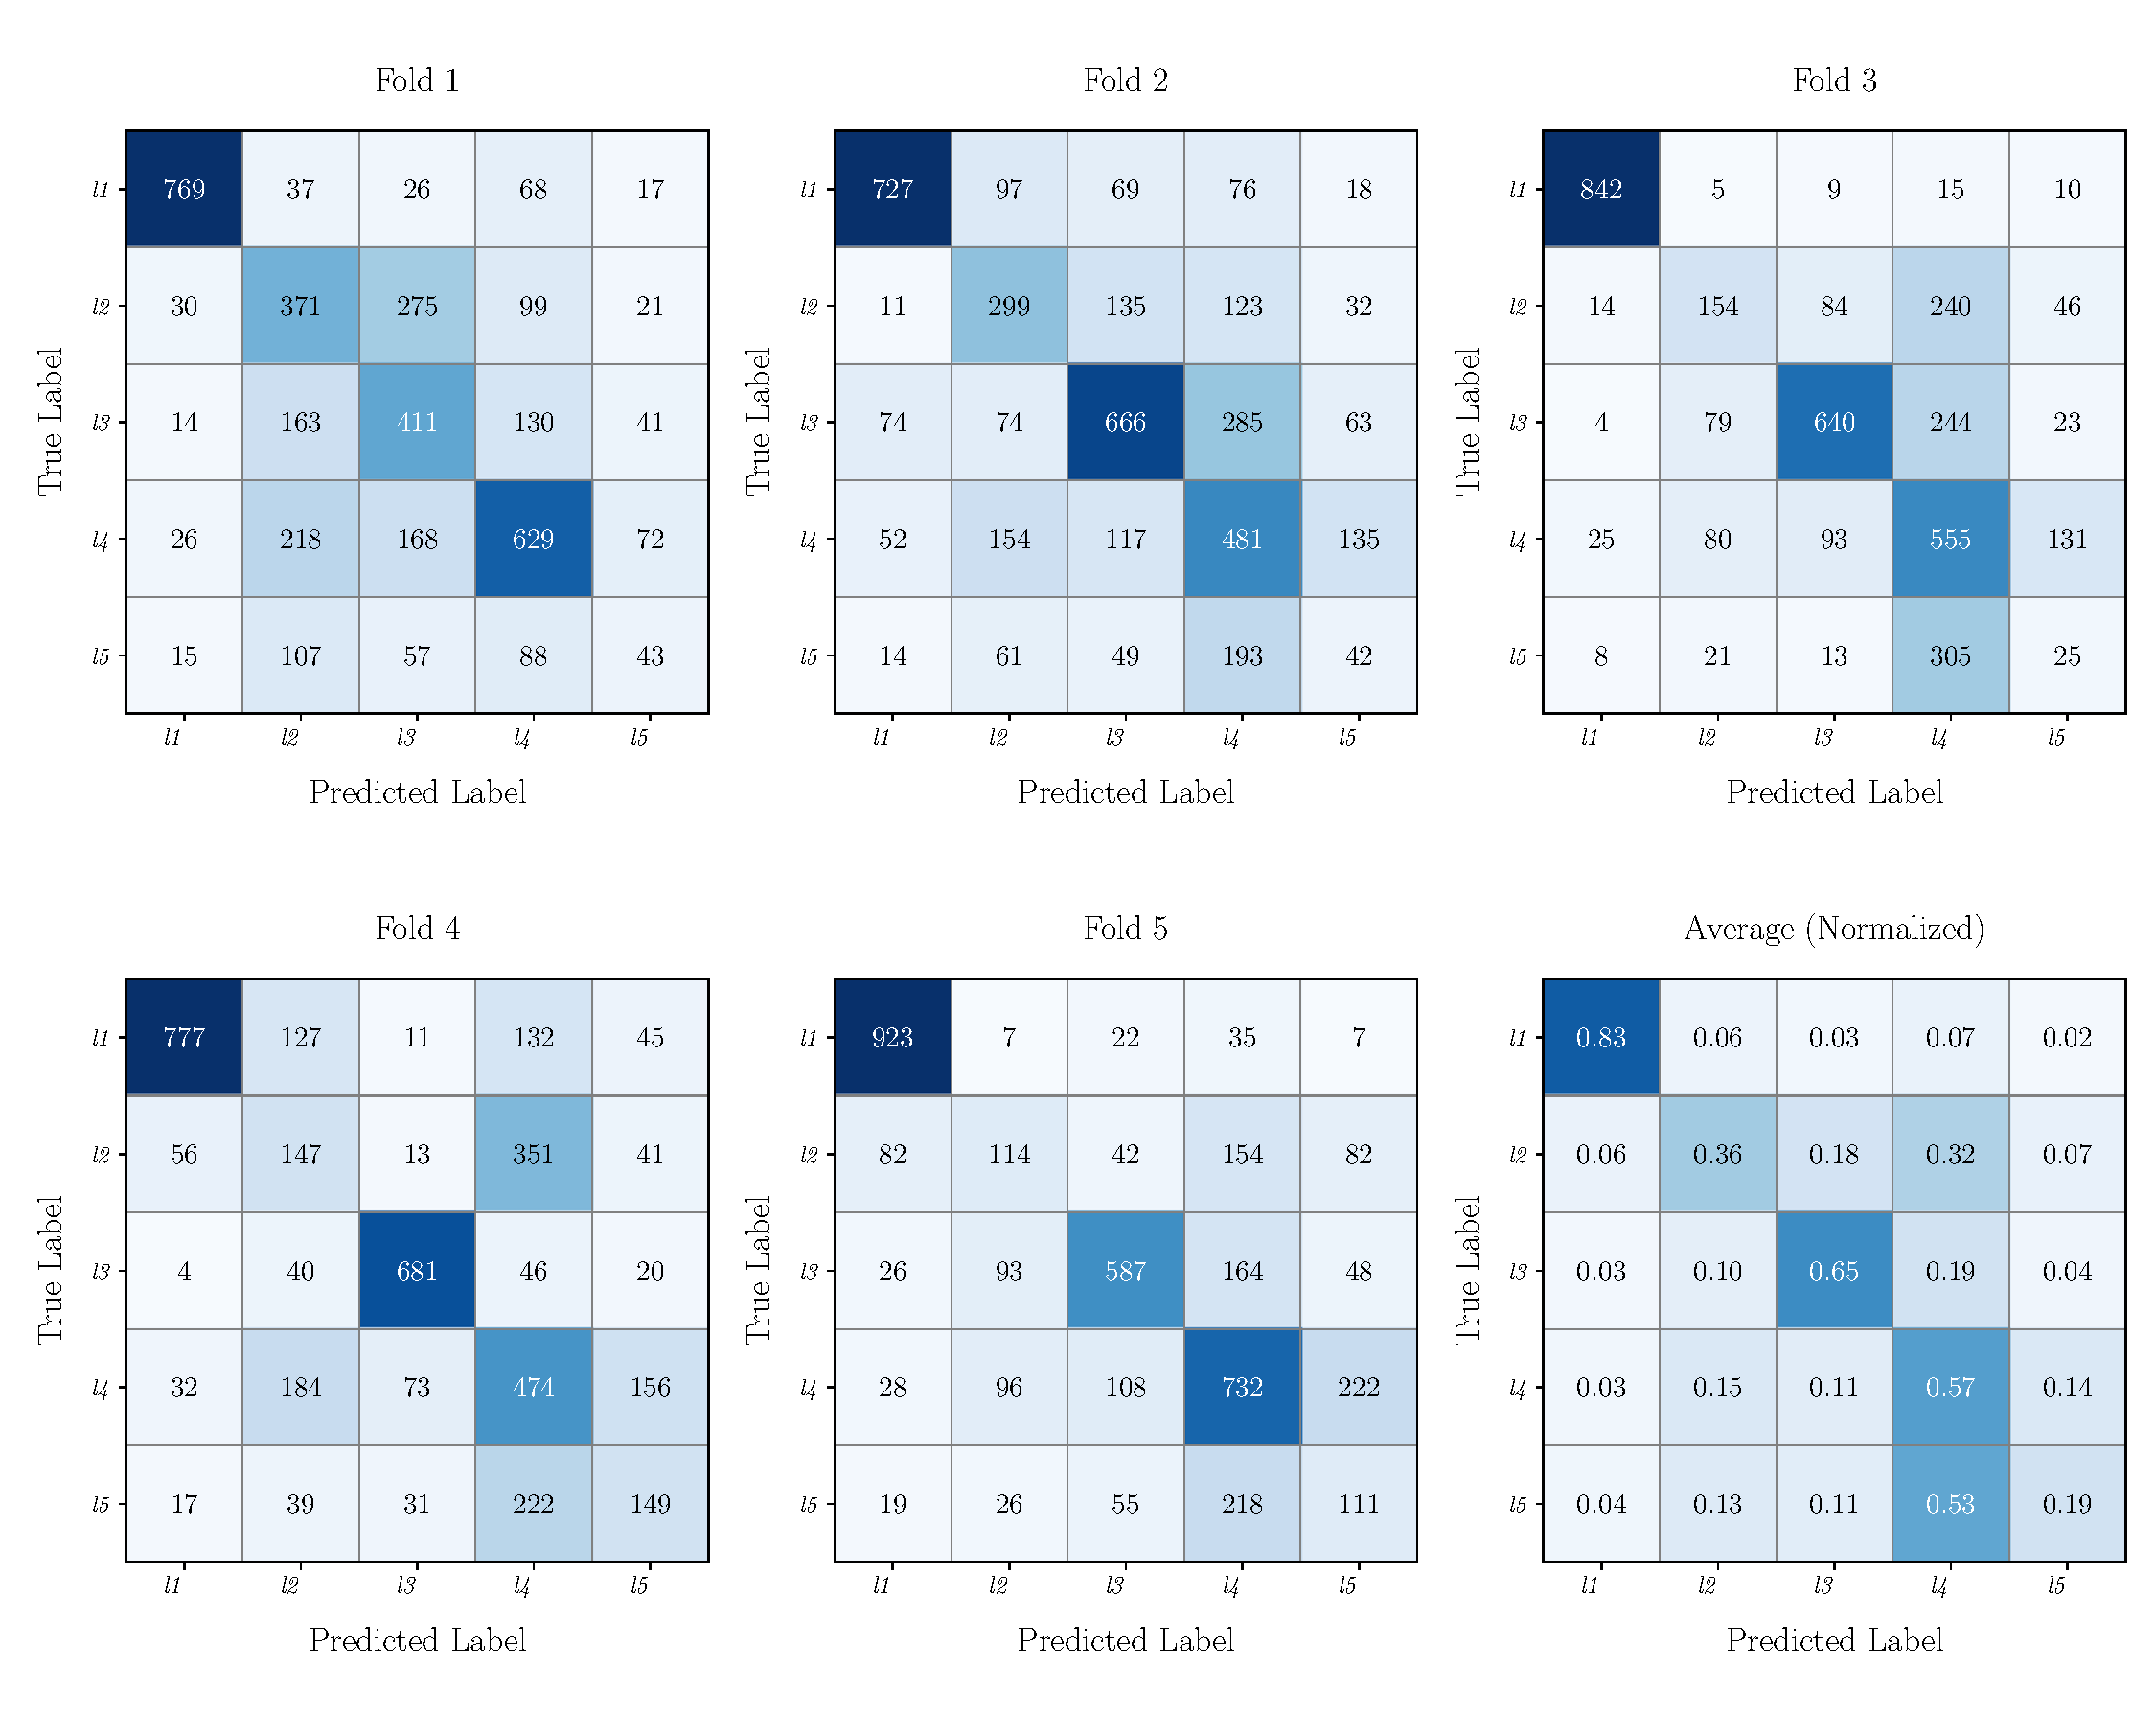
\includegraphics[width=\linewidth]{img/cm_bert.pdf}
  \caption{BERT}\label{fig:bert_cms}
\end{subfigure}\hfill
\begin{subfigure}[b]{0.48\linewidth}
  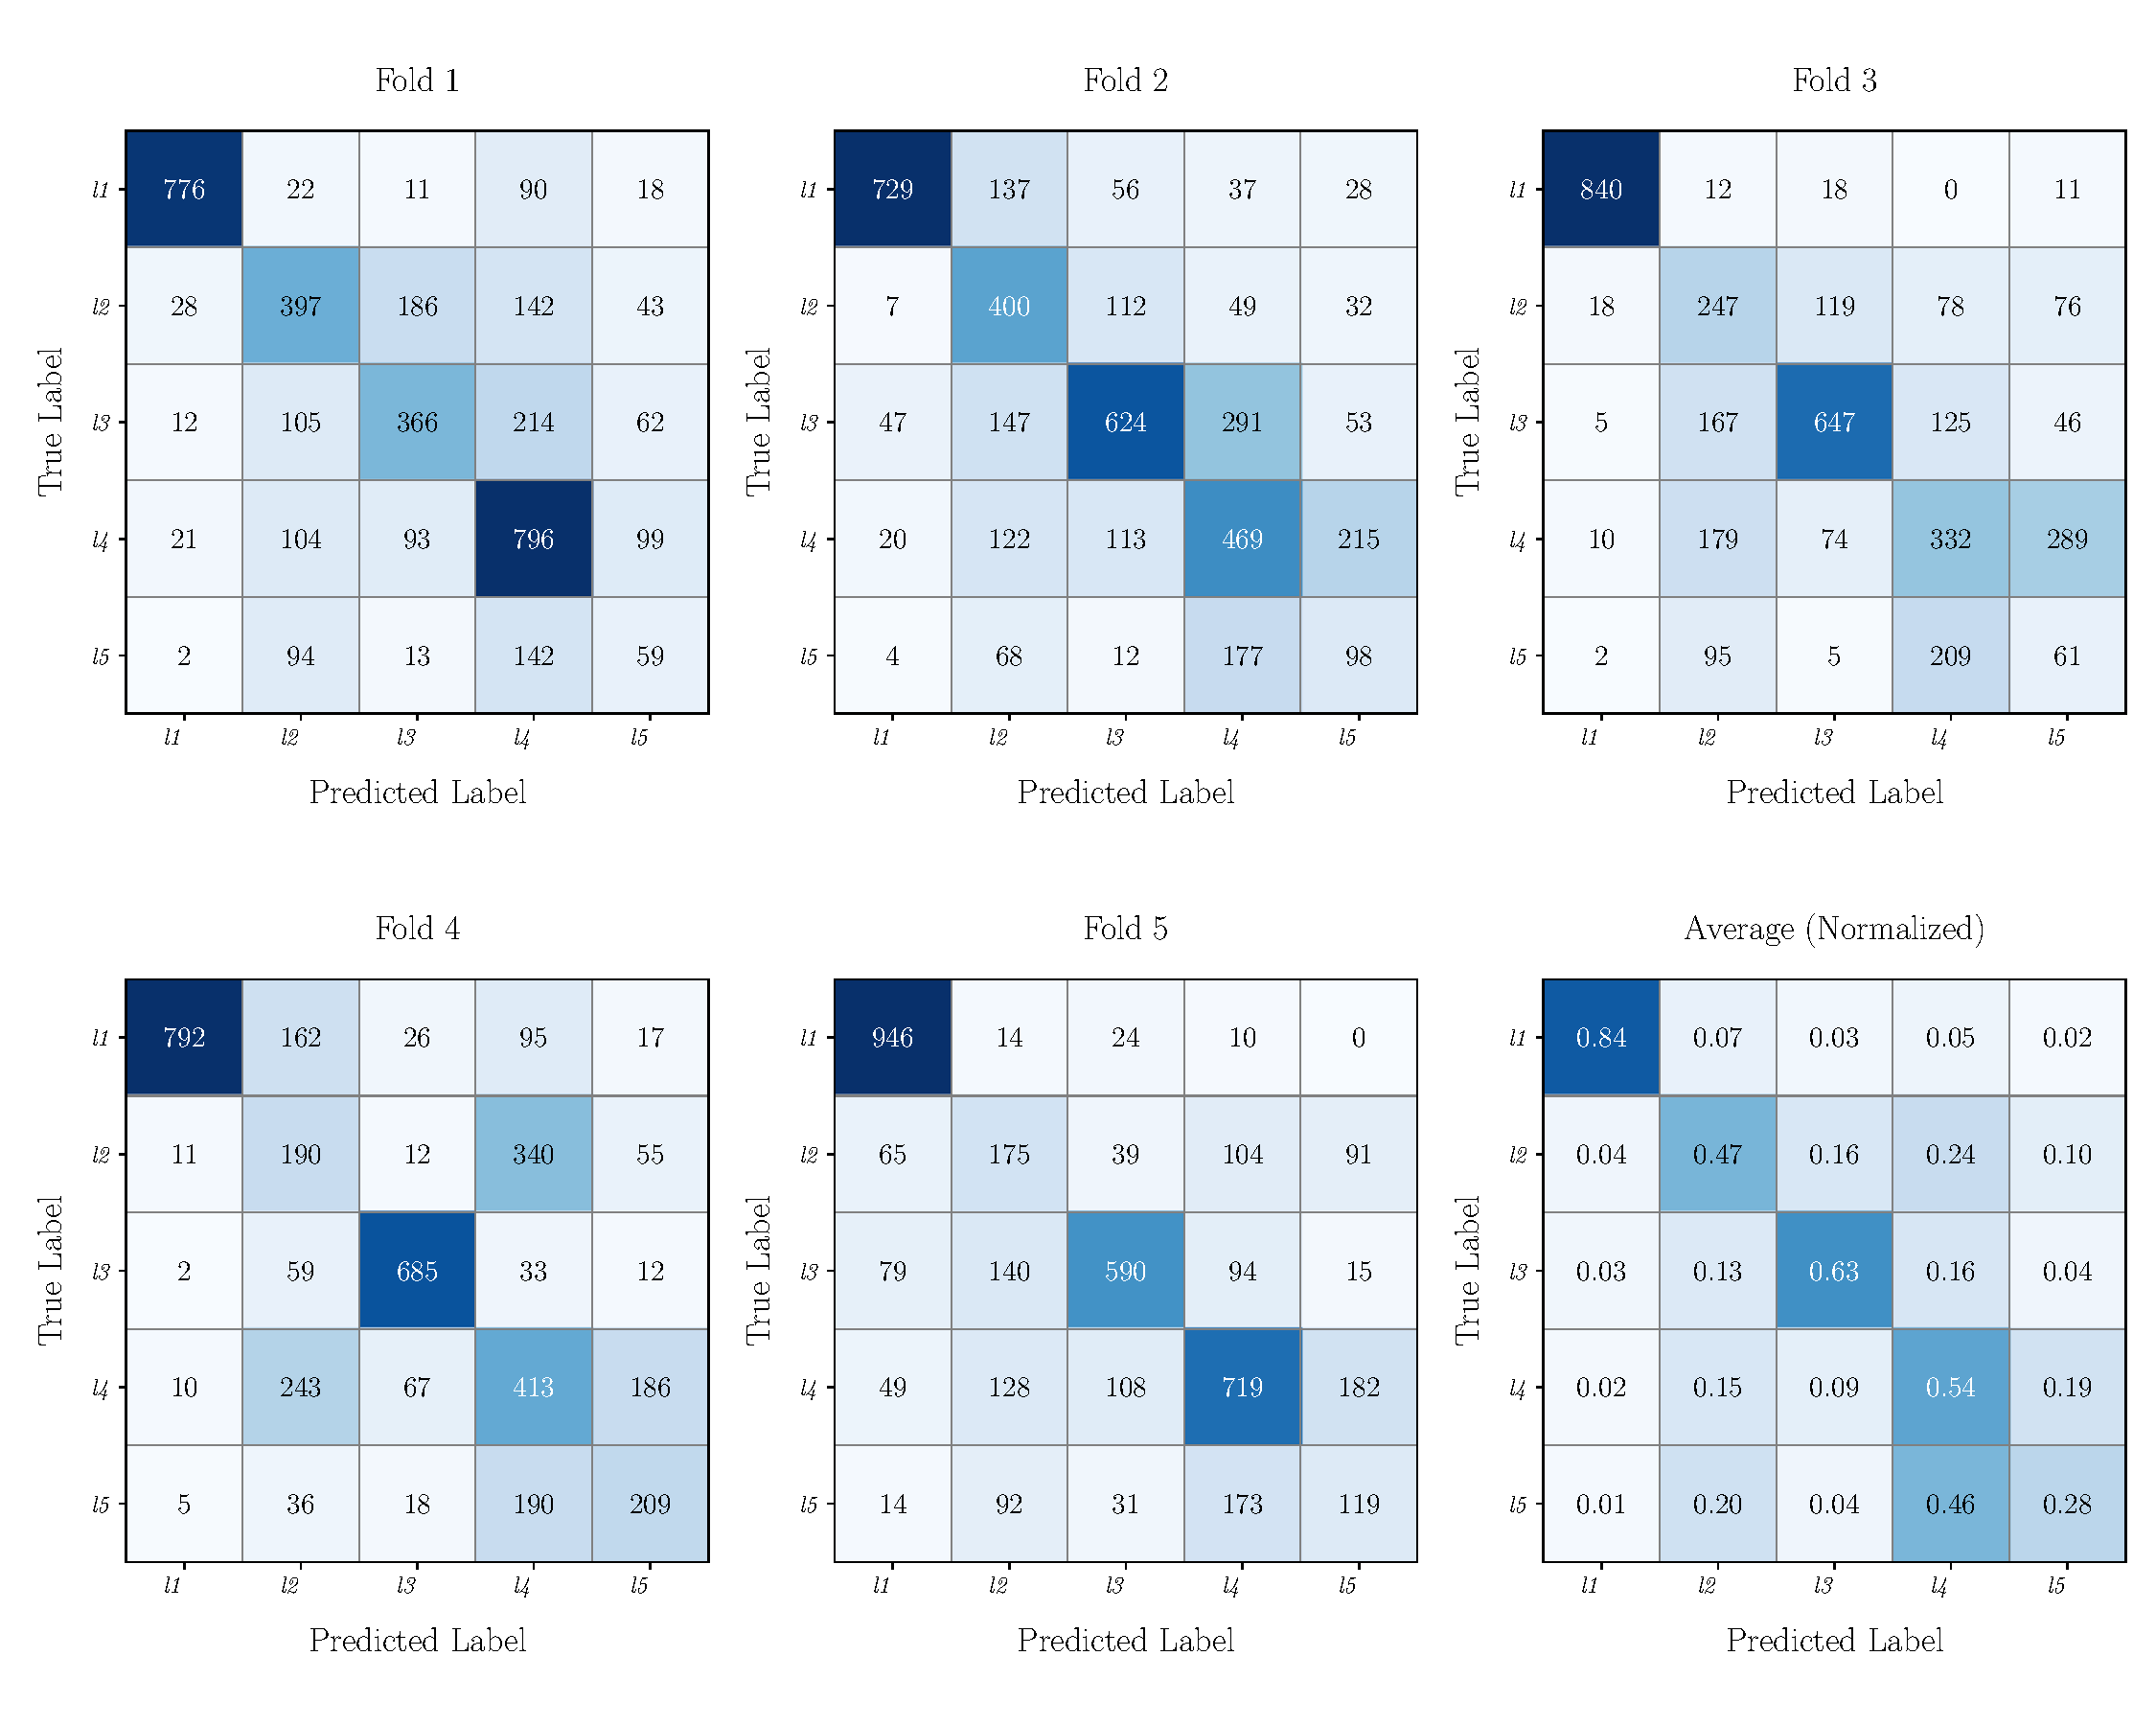
\includegraphics[width=\linewidth]{img/cm_roberta.pdf}
  \caption{RoBERTa}\label{fig:roberta_cms}
\end{subfigure}

\vspace{0.4cm}

\begin{subfigure}[b]{0.48\linewidth}
  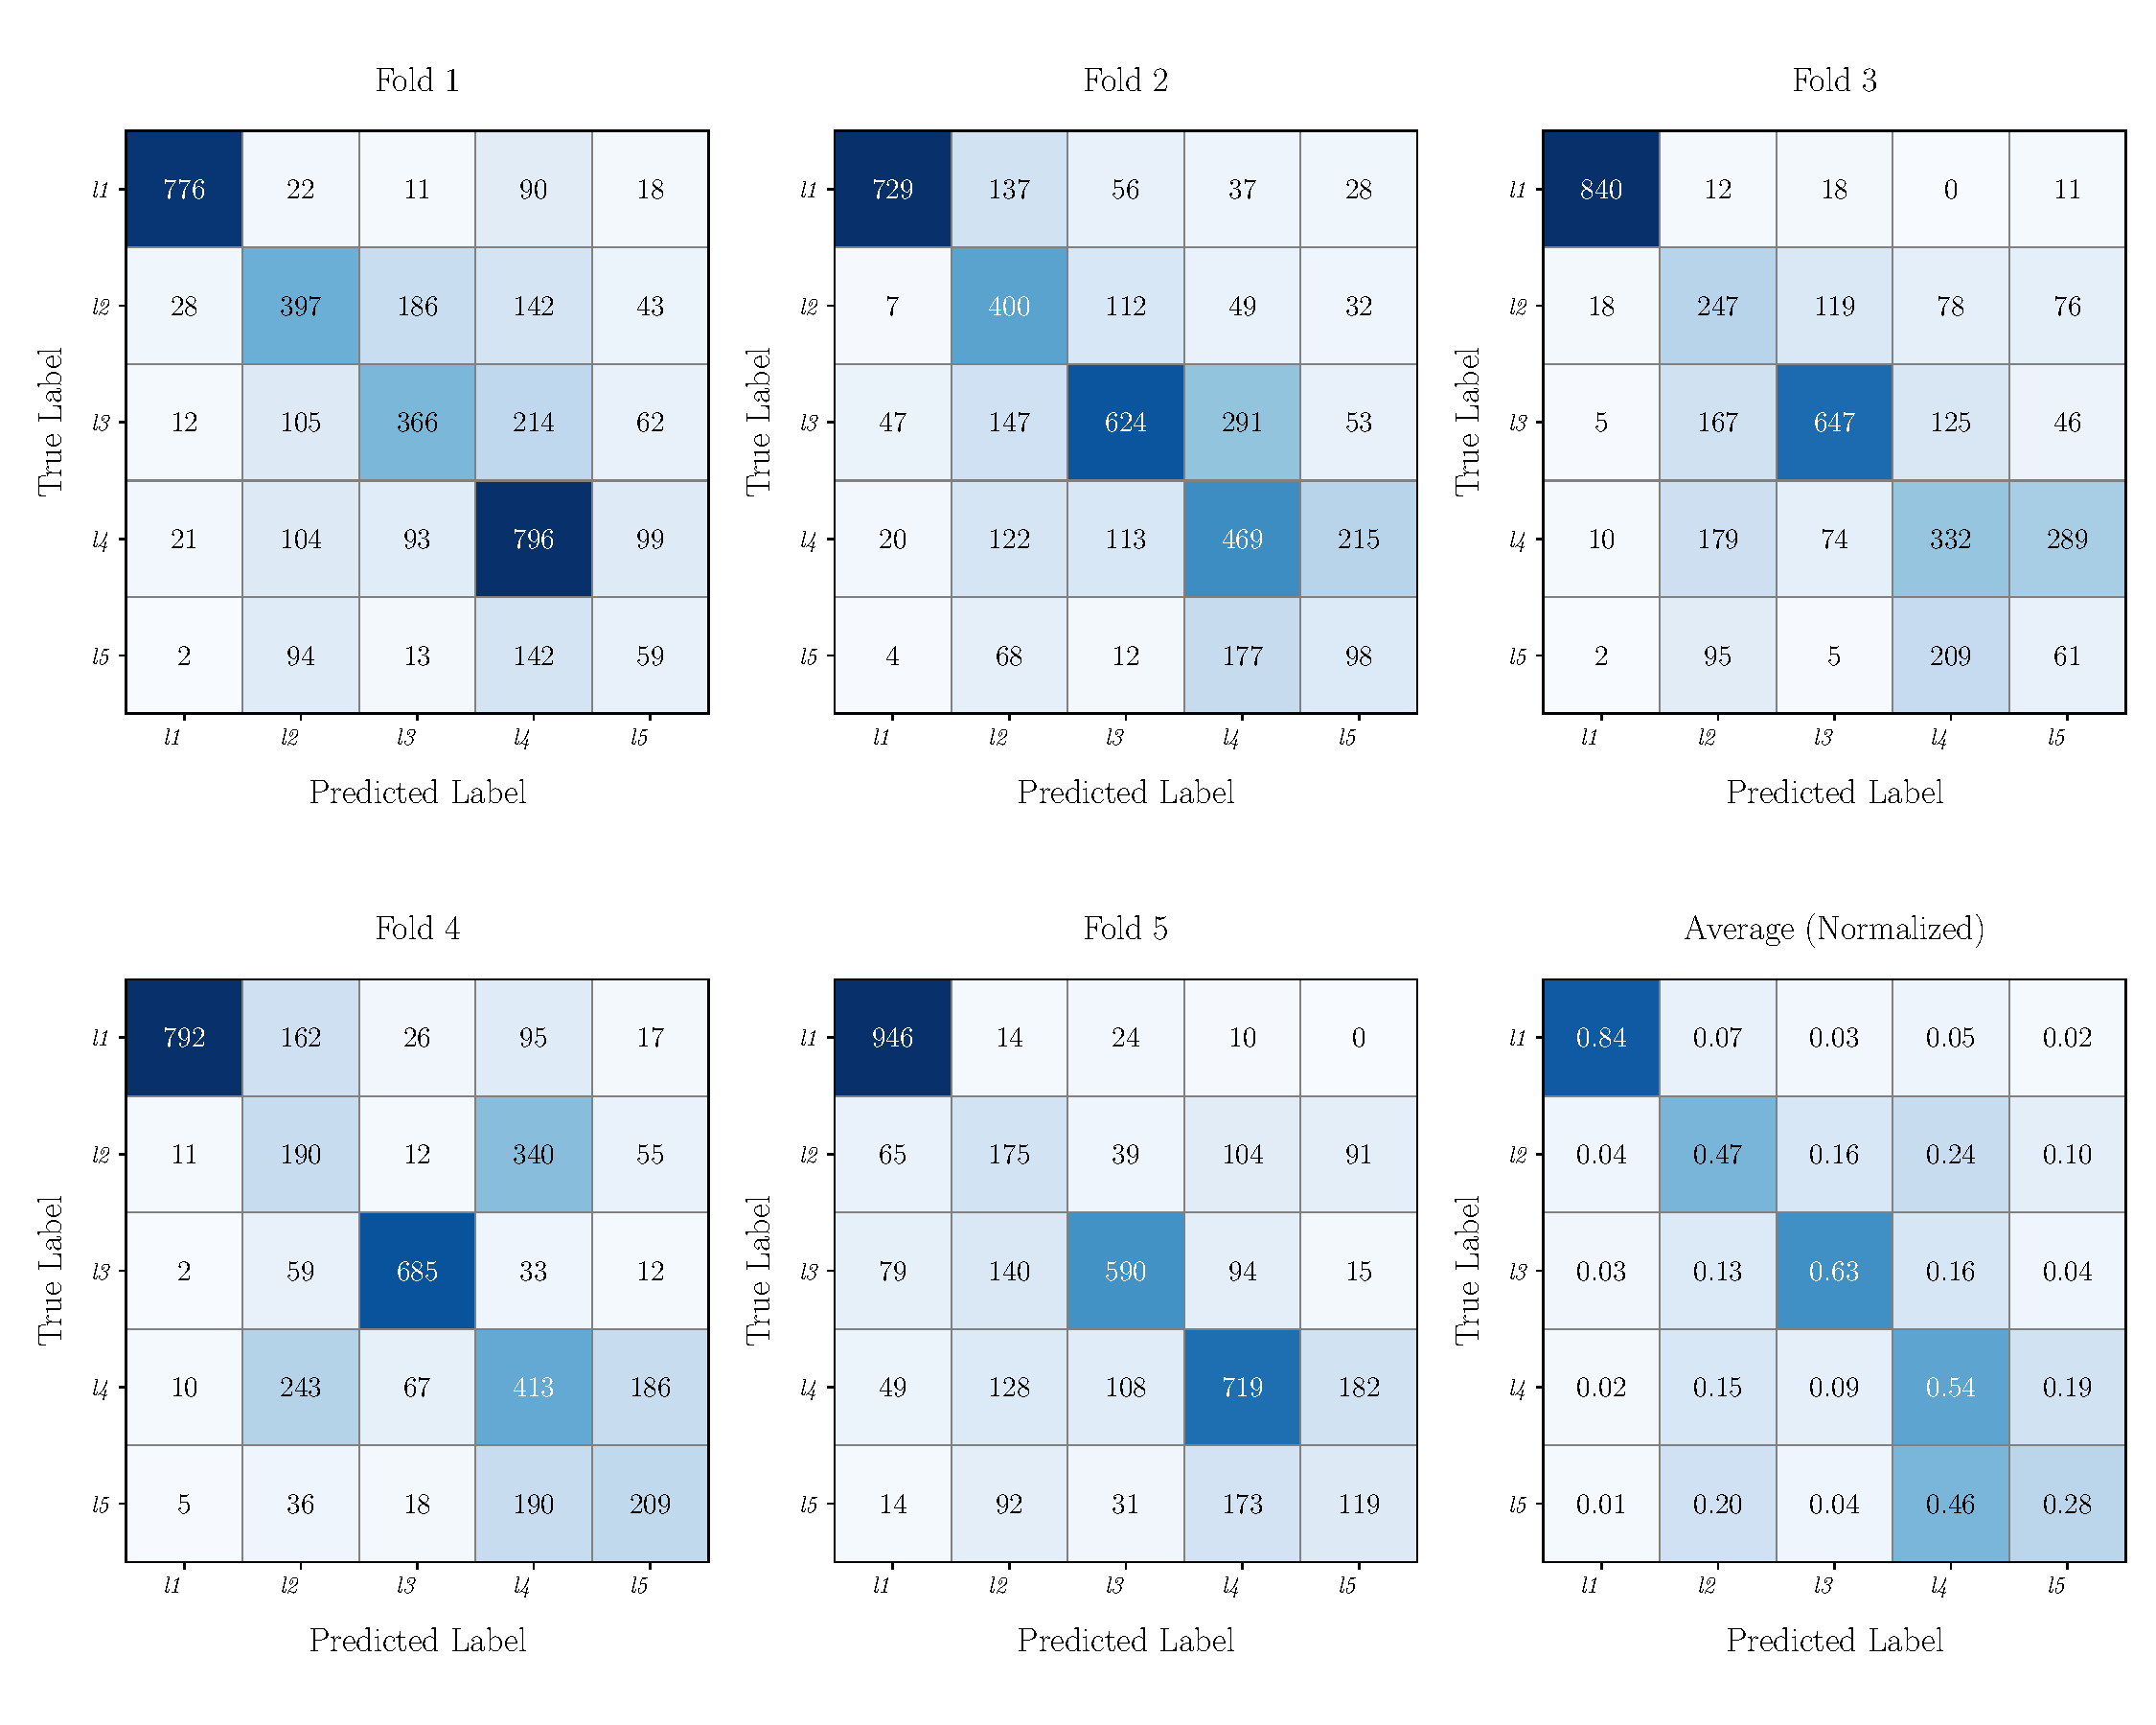
\includegraphics[width=\linewidth]{img/cm_llama.pdf}
  \caption{Llama 3}\label{fig:llama_cms}
\end{subfigure}\hfill
\begin{subfigure}[b]{0.48\linewidth}
  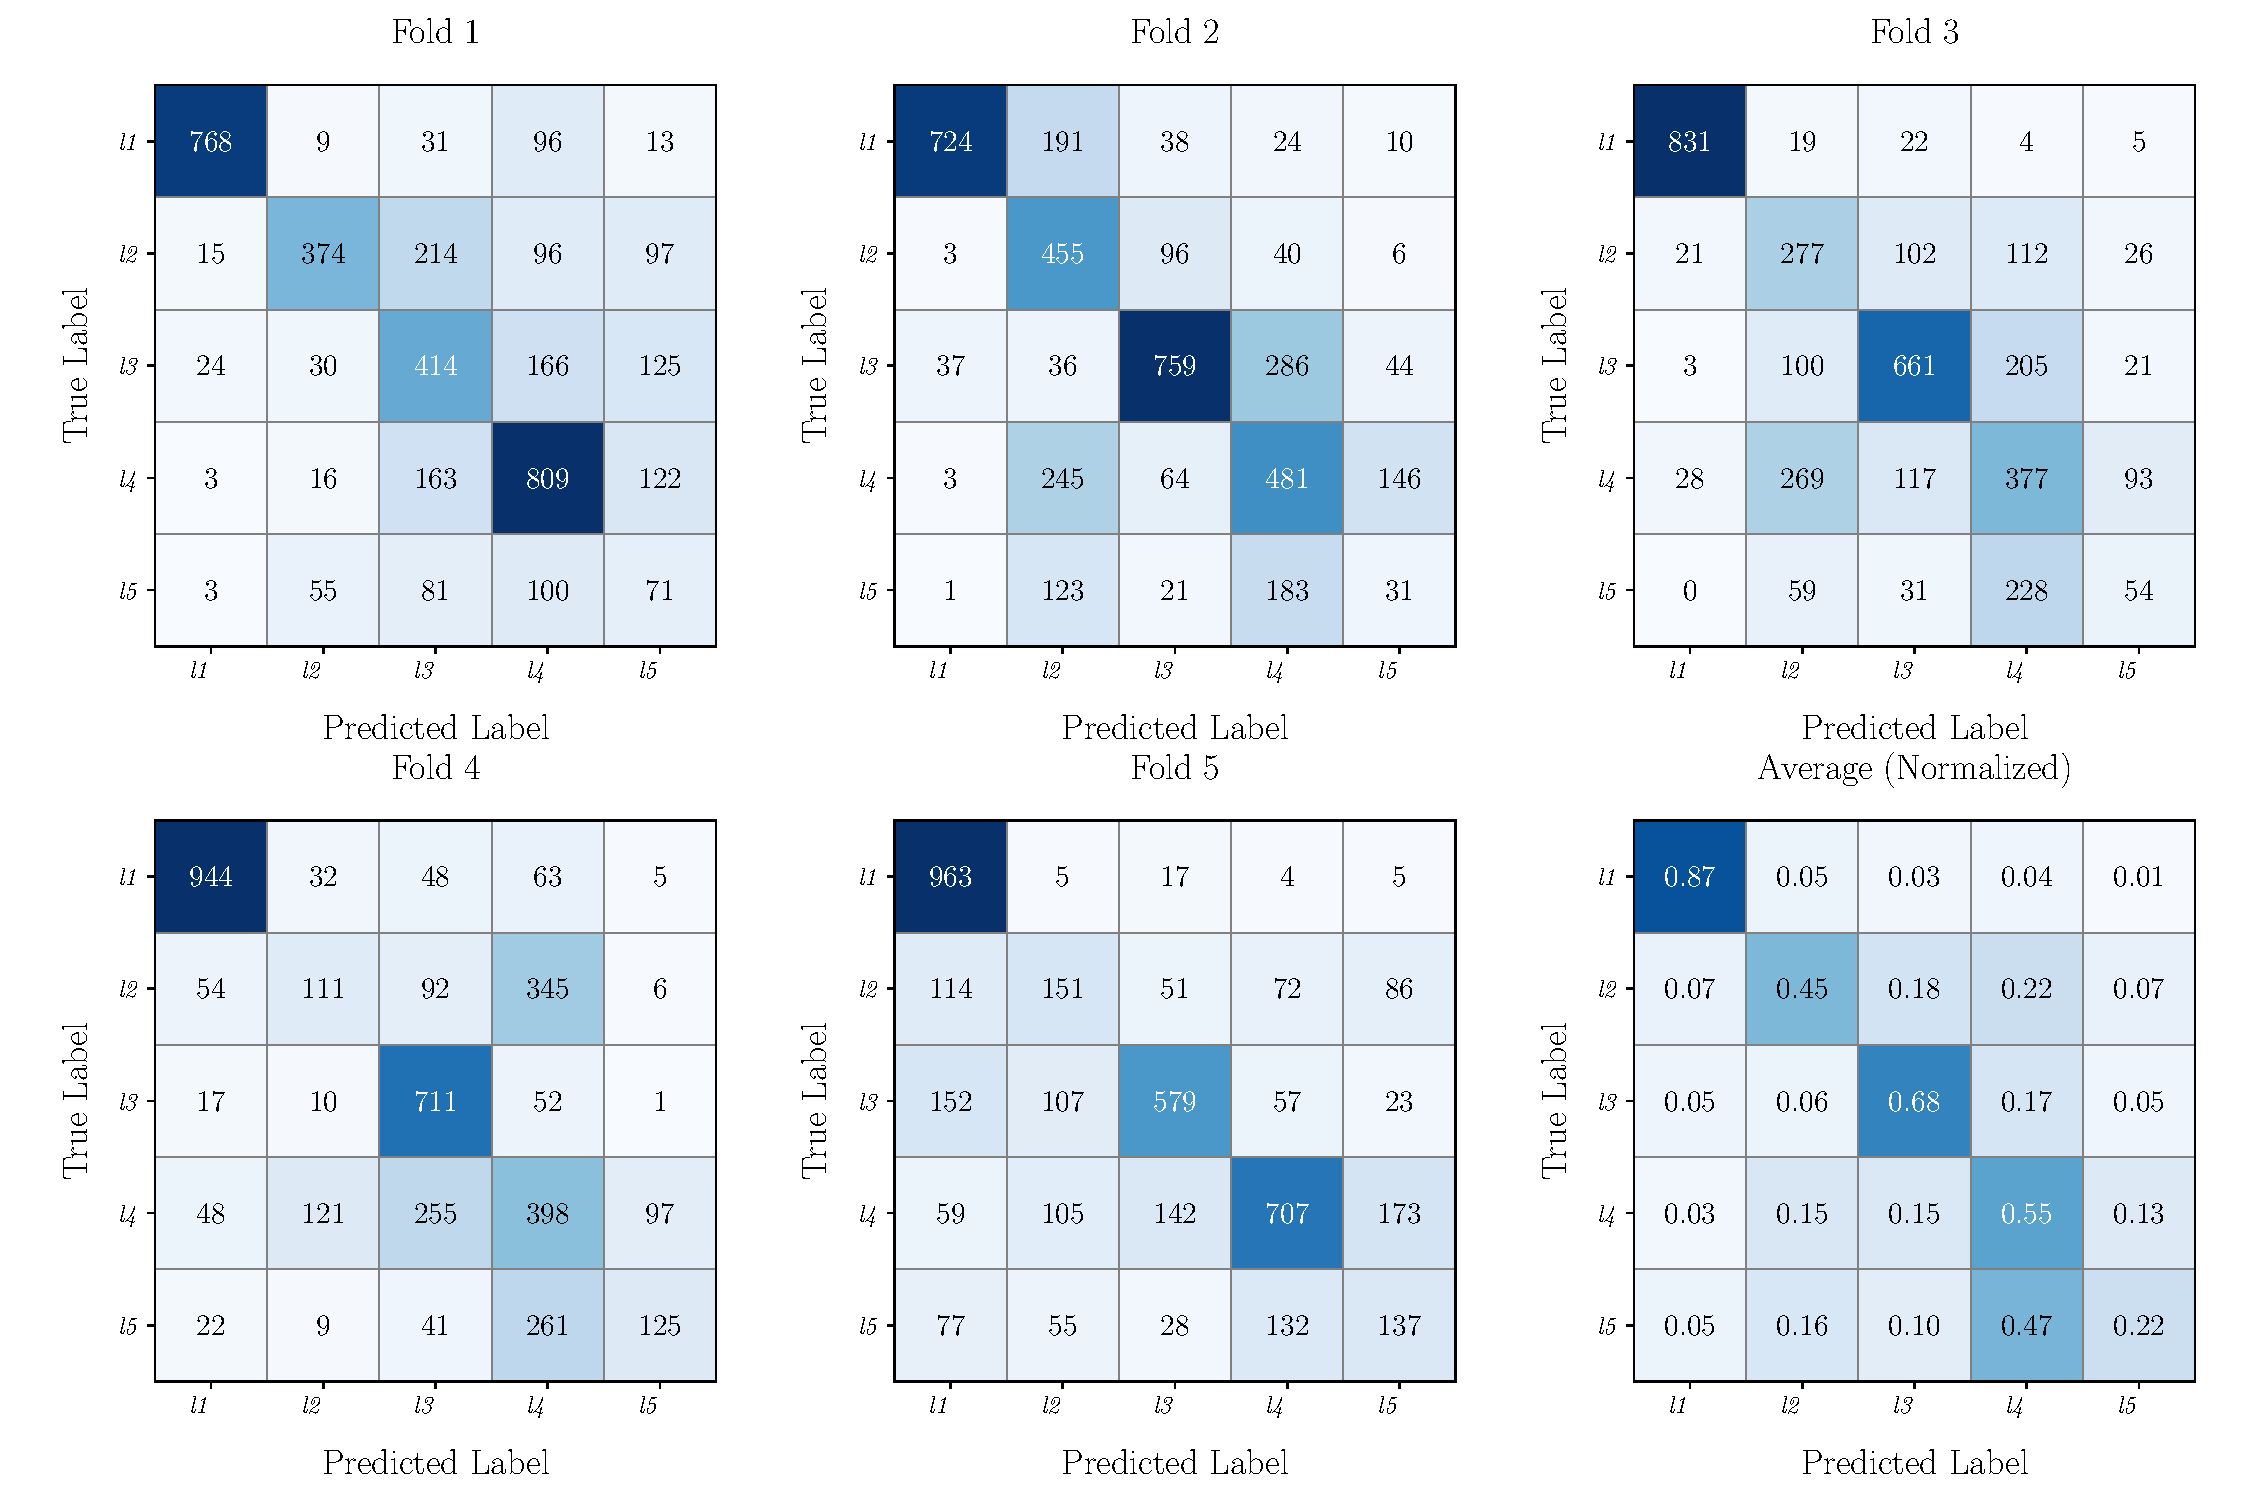
\includegraphics[width=\linewidth]{img/cm_mistral.pdf}
  \caption{Mistral}\label{fig:mistral_cms}
\end{subfigure}

\caption{Confusion matrices showing the models' performance across five cross-validation folds and their overall average. The rows correspond to the true labels and the columns to the predicted ones.}
\label{fig:performance_cms}
\end{figure*}


\section{Publisher-level Results}
\label{app:publisher_cms}

Figure~\ref{fig:publisher_cms} reports the publisher-level confusion matrices obtained after aggregating article-level predictions by majority voting.

\begin{figure*}[!t]
\centering
\begin{subfigure}[b]{0.24\linewidth}
  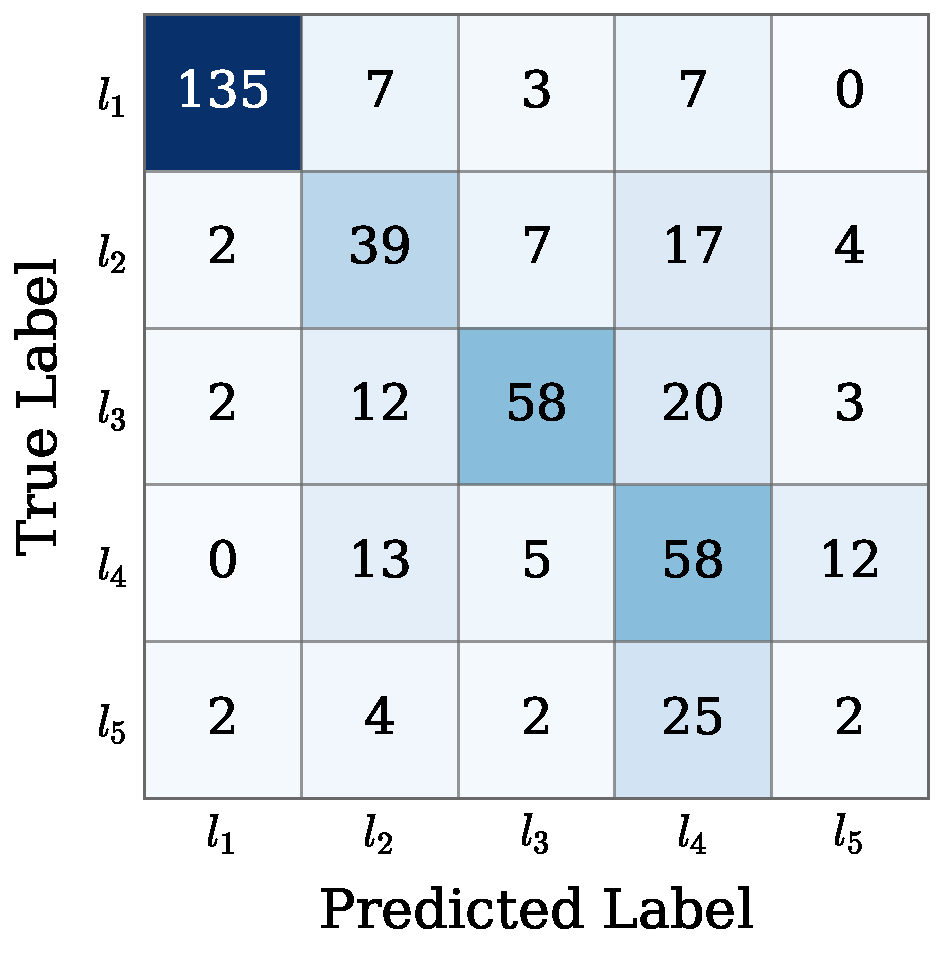
\includegraphics[width=\linewidth]{img/domain_confusion_matrix_bert.pdf}
  \caption{BERT}\label{fig:pub_bert}
\end{subfigure}\hfill
\begin{subfigure}[b]{0.24\linewidth}
  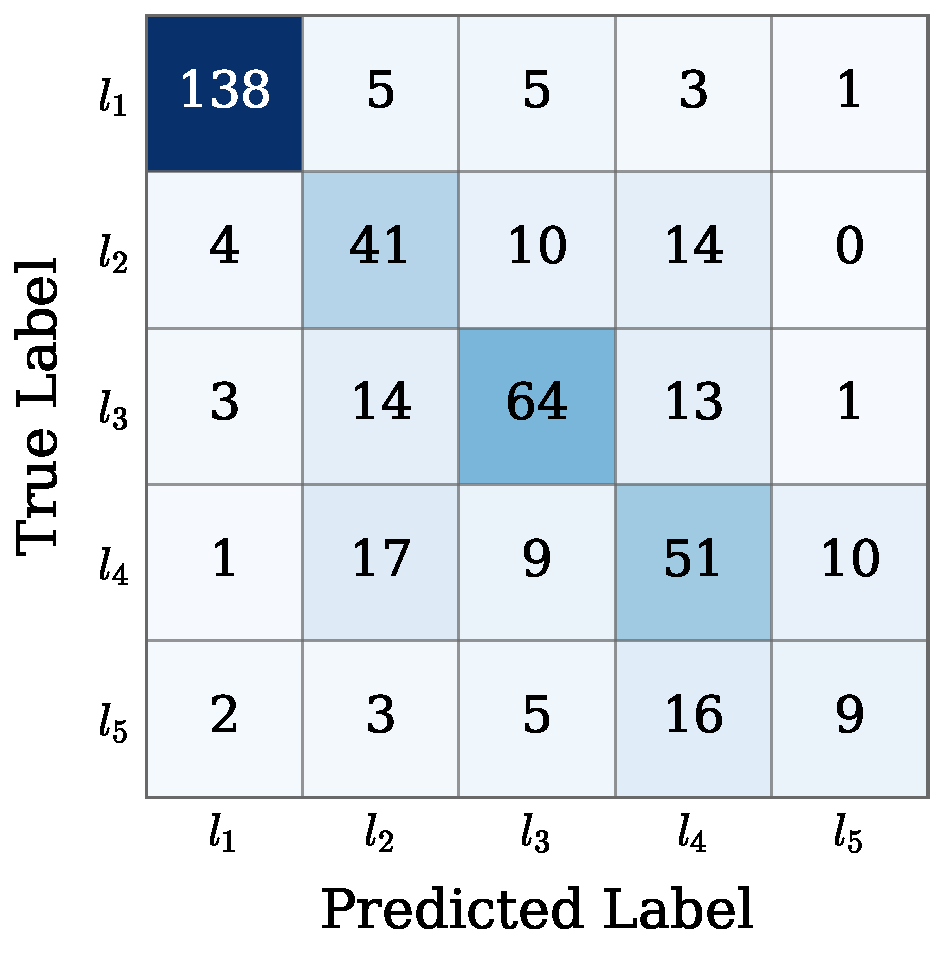
\includegraphics[width=\linewidth]{img/domain_confusion_matrix_roberta.pdf}
  \caption{RoBERTa}\label{fig:pub_roberta}
\end{subfigure}\hfill
\begin{subfigure}[b]{0.24\linewidth}
  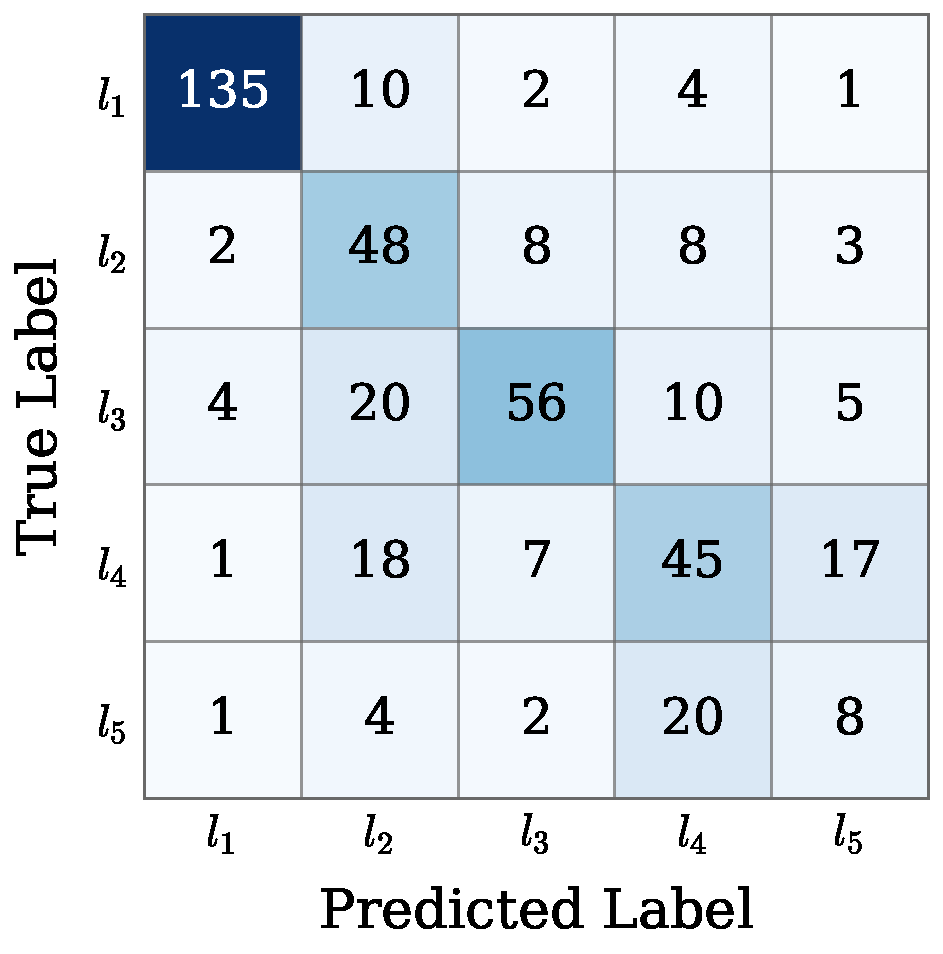
\includegraphics[width=\linewidth]{img/domain_confusion_matrix_llama.pdf}
  \caption{Llama 3}\label{fig:pub_llama}
\end{subfigure}\hfill
\begin{subfigure}[b]{0.24\linewidth}
  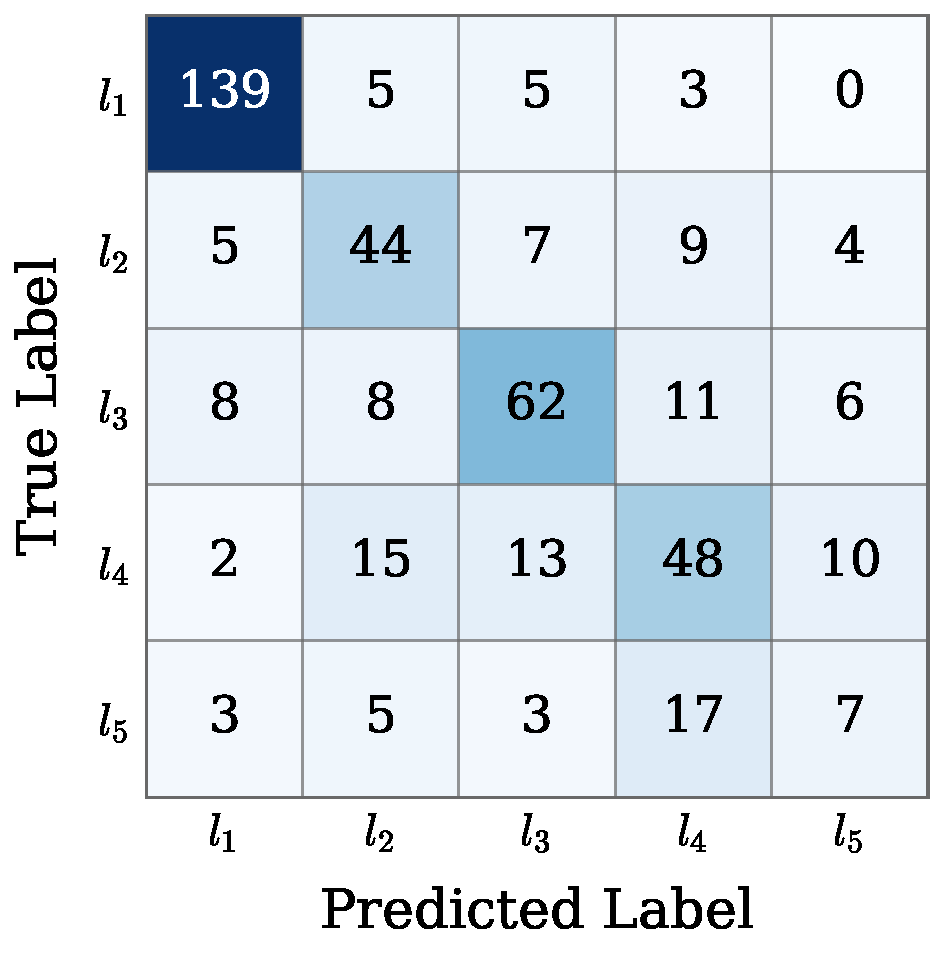
\includegraphics[width=\linewidth]{img/domain_confusion_matrix_mistral.pdf}
  \caption{Mistral}\label{fig:pub_mistral}
\end{subfigure}
\caption{Publisher-level confusion matrices for BERT, RoBERTa, Llama 3, and Mistral. Rows indicate true reliability levels, columns indicate predicted levels.}
\label{fig:publisher_cms}
\end{figure*}

The matrices reveal that errors are strictly local. The most frequent confusion occurs between $l_4$ (Generally Credible) and $l_5$ (High Credibility). As observed at the article level, distinguishing $l_5$ from $l_4$ is inherently difficult because $l_5$ represents a strict ceiling (score = 100) while $l_4$ covers the immediately lower high-credibility range (75--99). Misclassifying these two adjacent levels constitutes a minor severity error, as both indicate high reliability. No model exhibits systematic confusion across non-adjacent levels, confirming that aggregation stabilizes predictions.

One caveat applies to every publisher-level number reported here and in the main paper. Aggregation is a majority vote, and ties are resolved deterministically in favour of the \emph{lowest} reliability level. This affects a small but non-negligible share of publishers -- 13 of 439 for BERT, 20 for RoBERTa, 15 for Llama~3 and 11 for Mistral -- and always in the same direction, so it is a mild systematic pull toward lower predicted reliability rather than a neutral rule.


\section{Political leaning}
\label{app:political_cms}

\begin{figure*}[!t]
\centering
% --- row 1 ---
\begin{subfigure}[b]{0.48\linewidth}
  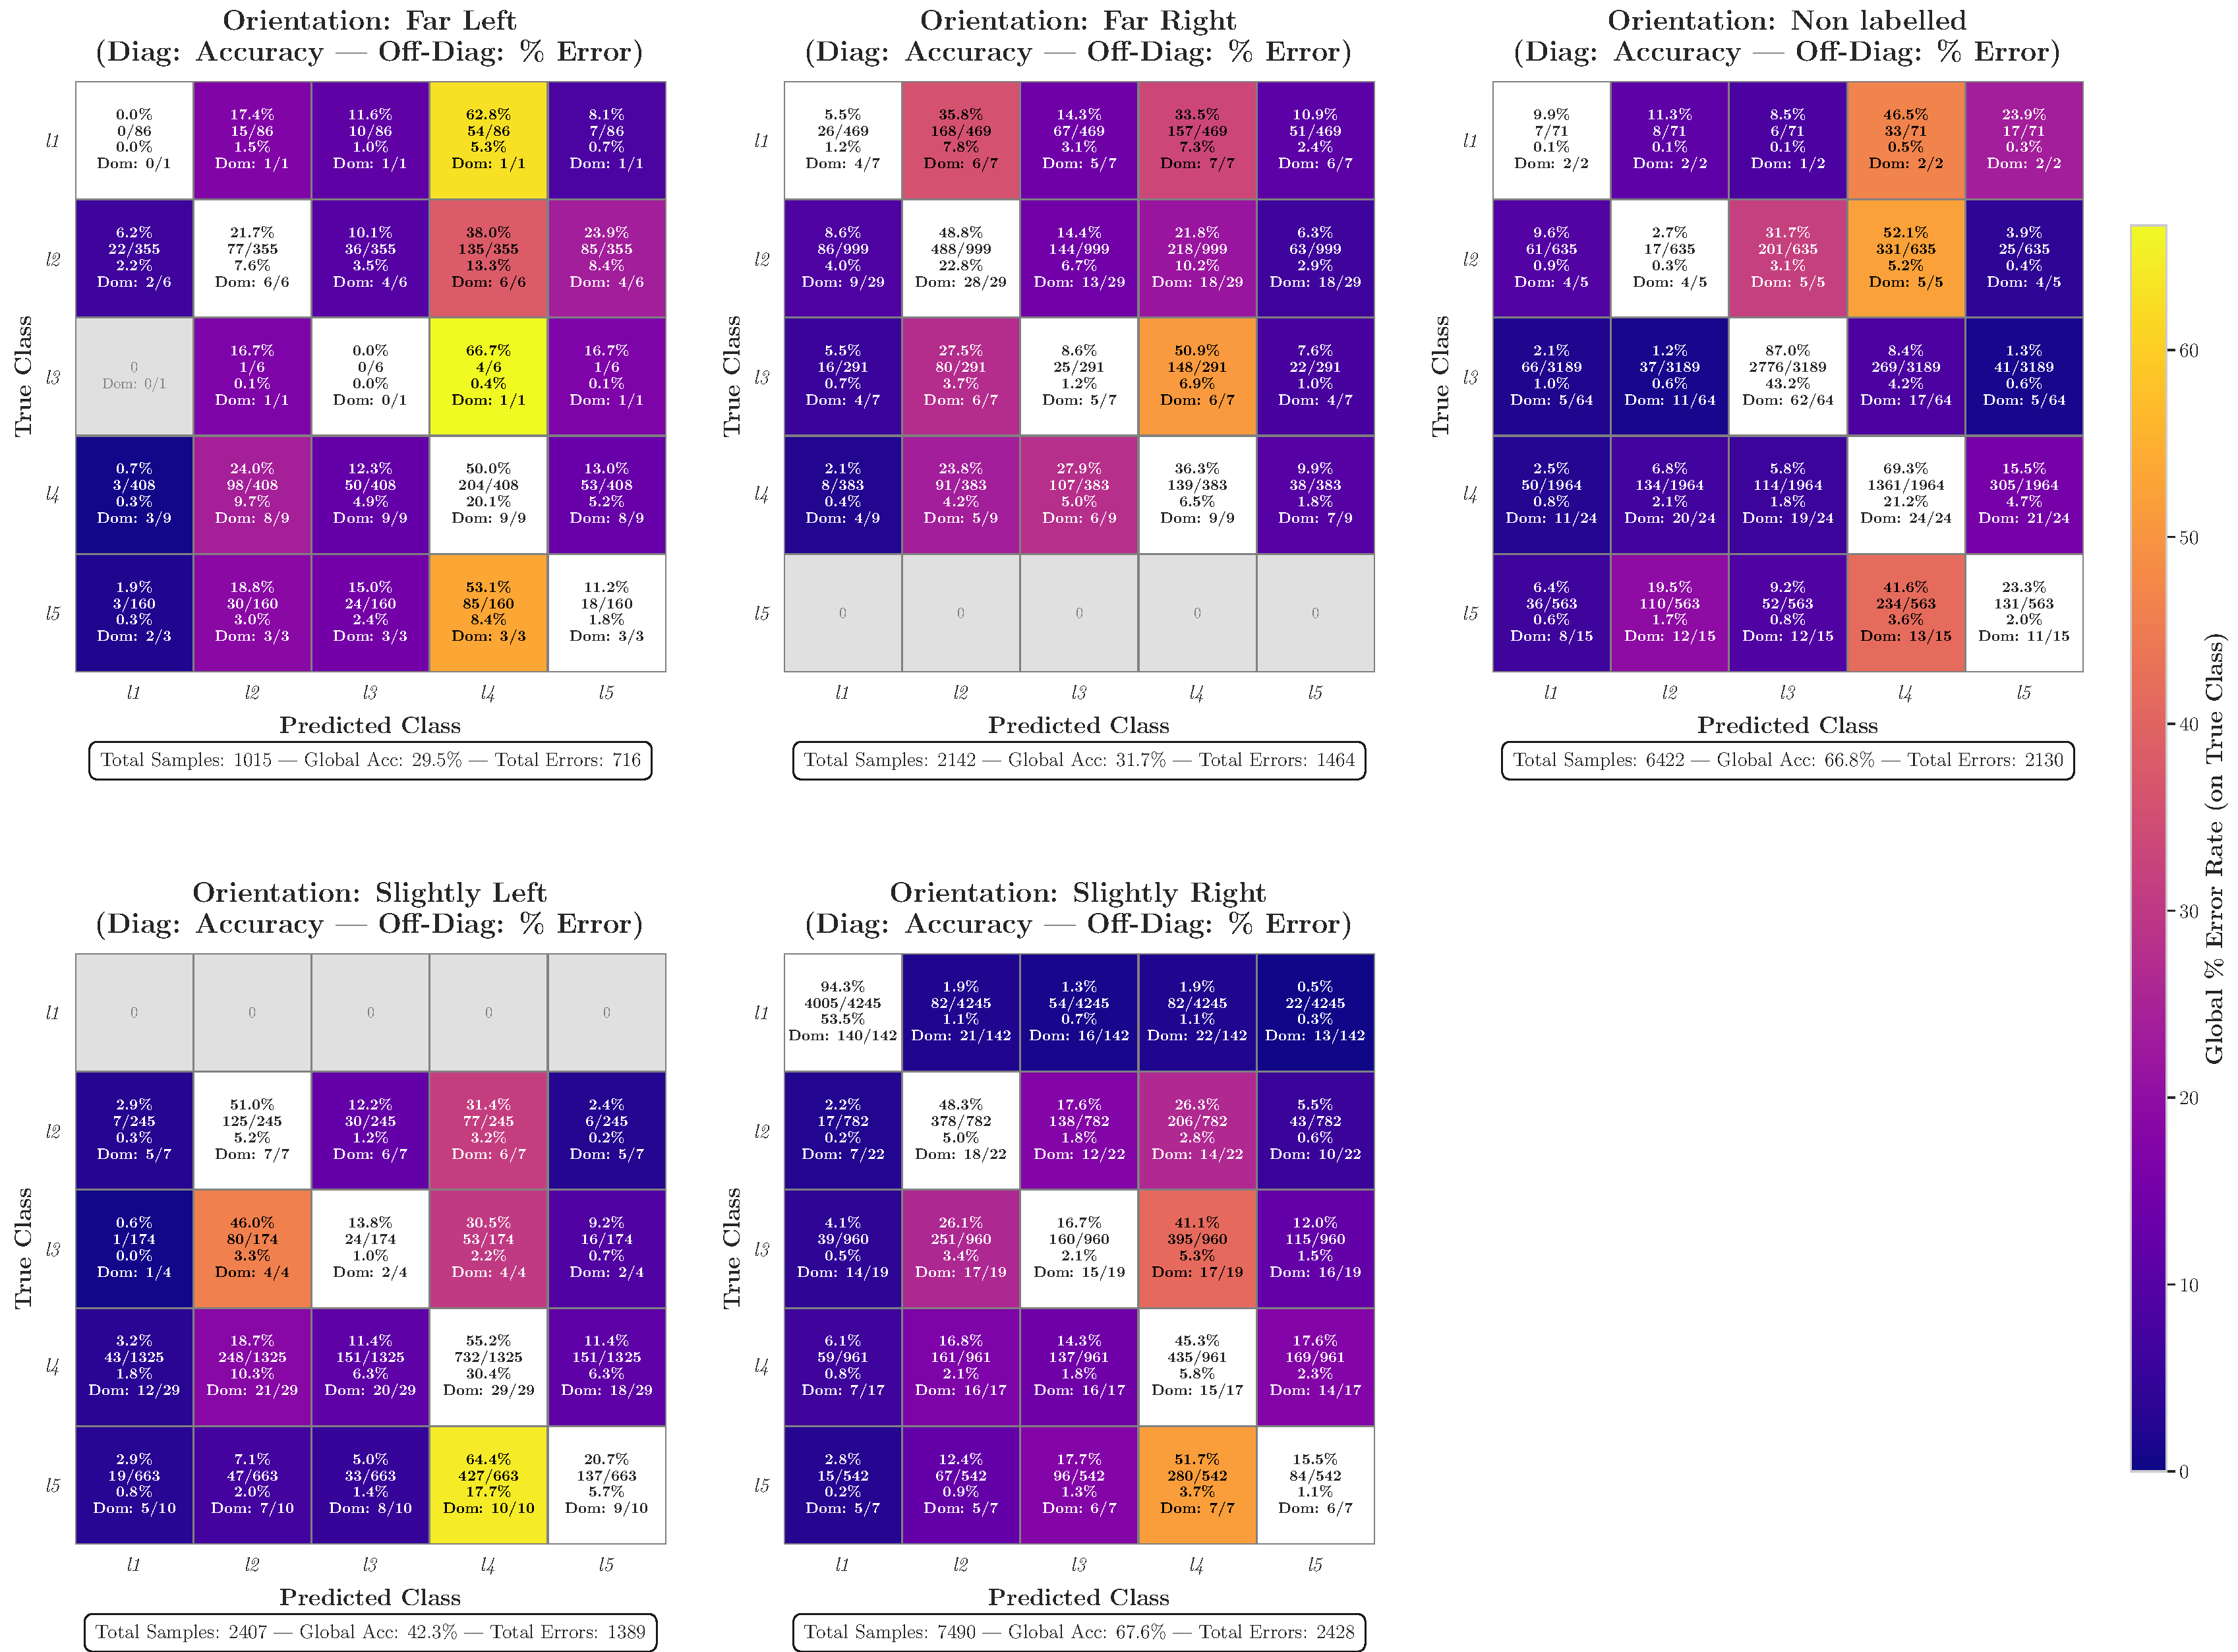
\includegraphics[width=\linewidth]{img/cmOnPoliticalLeaningBert.pdf}
  \caption{BERT}
  \label{fig:cmPoliticalLeaningBert}
\end{subfigure}\hfill
\begin{subfigure}[b]{0.48\linewidth}
  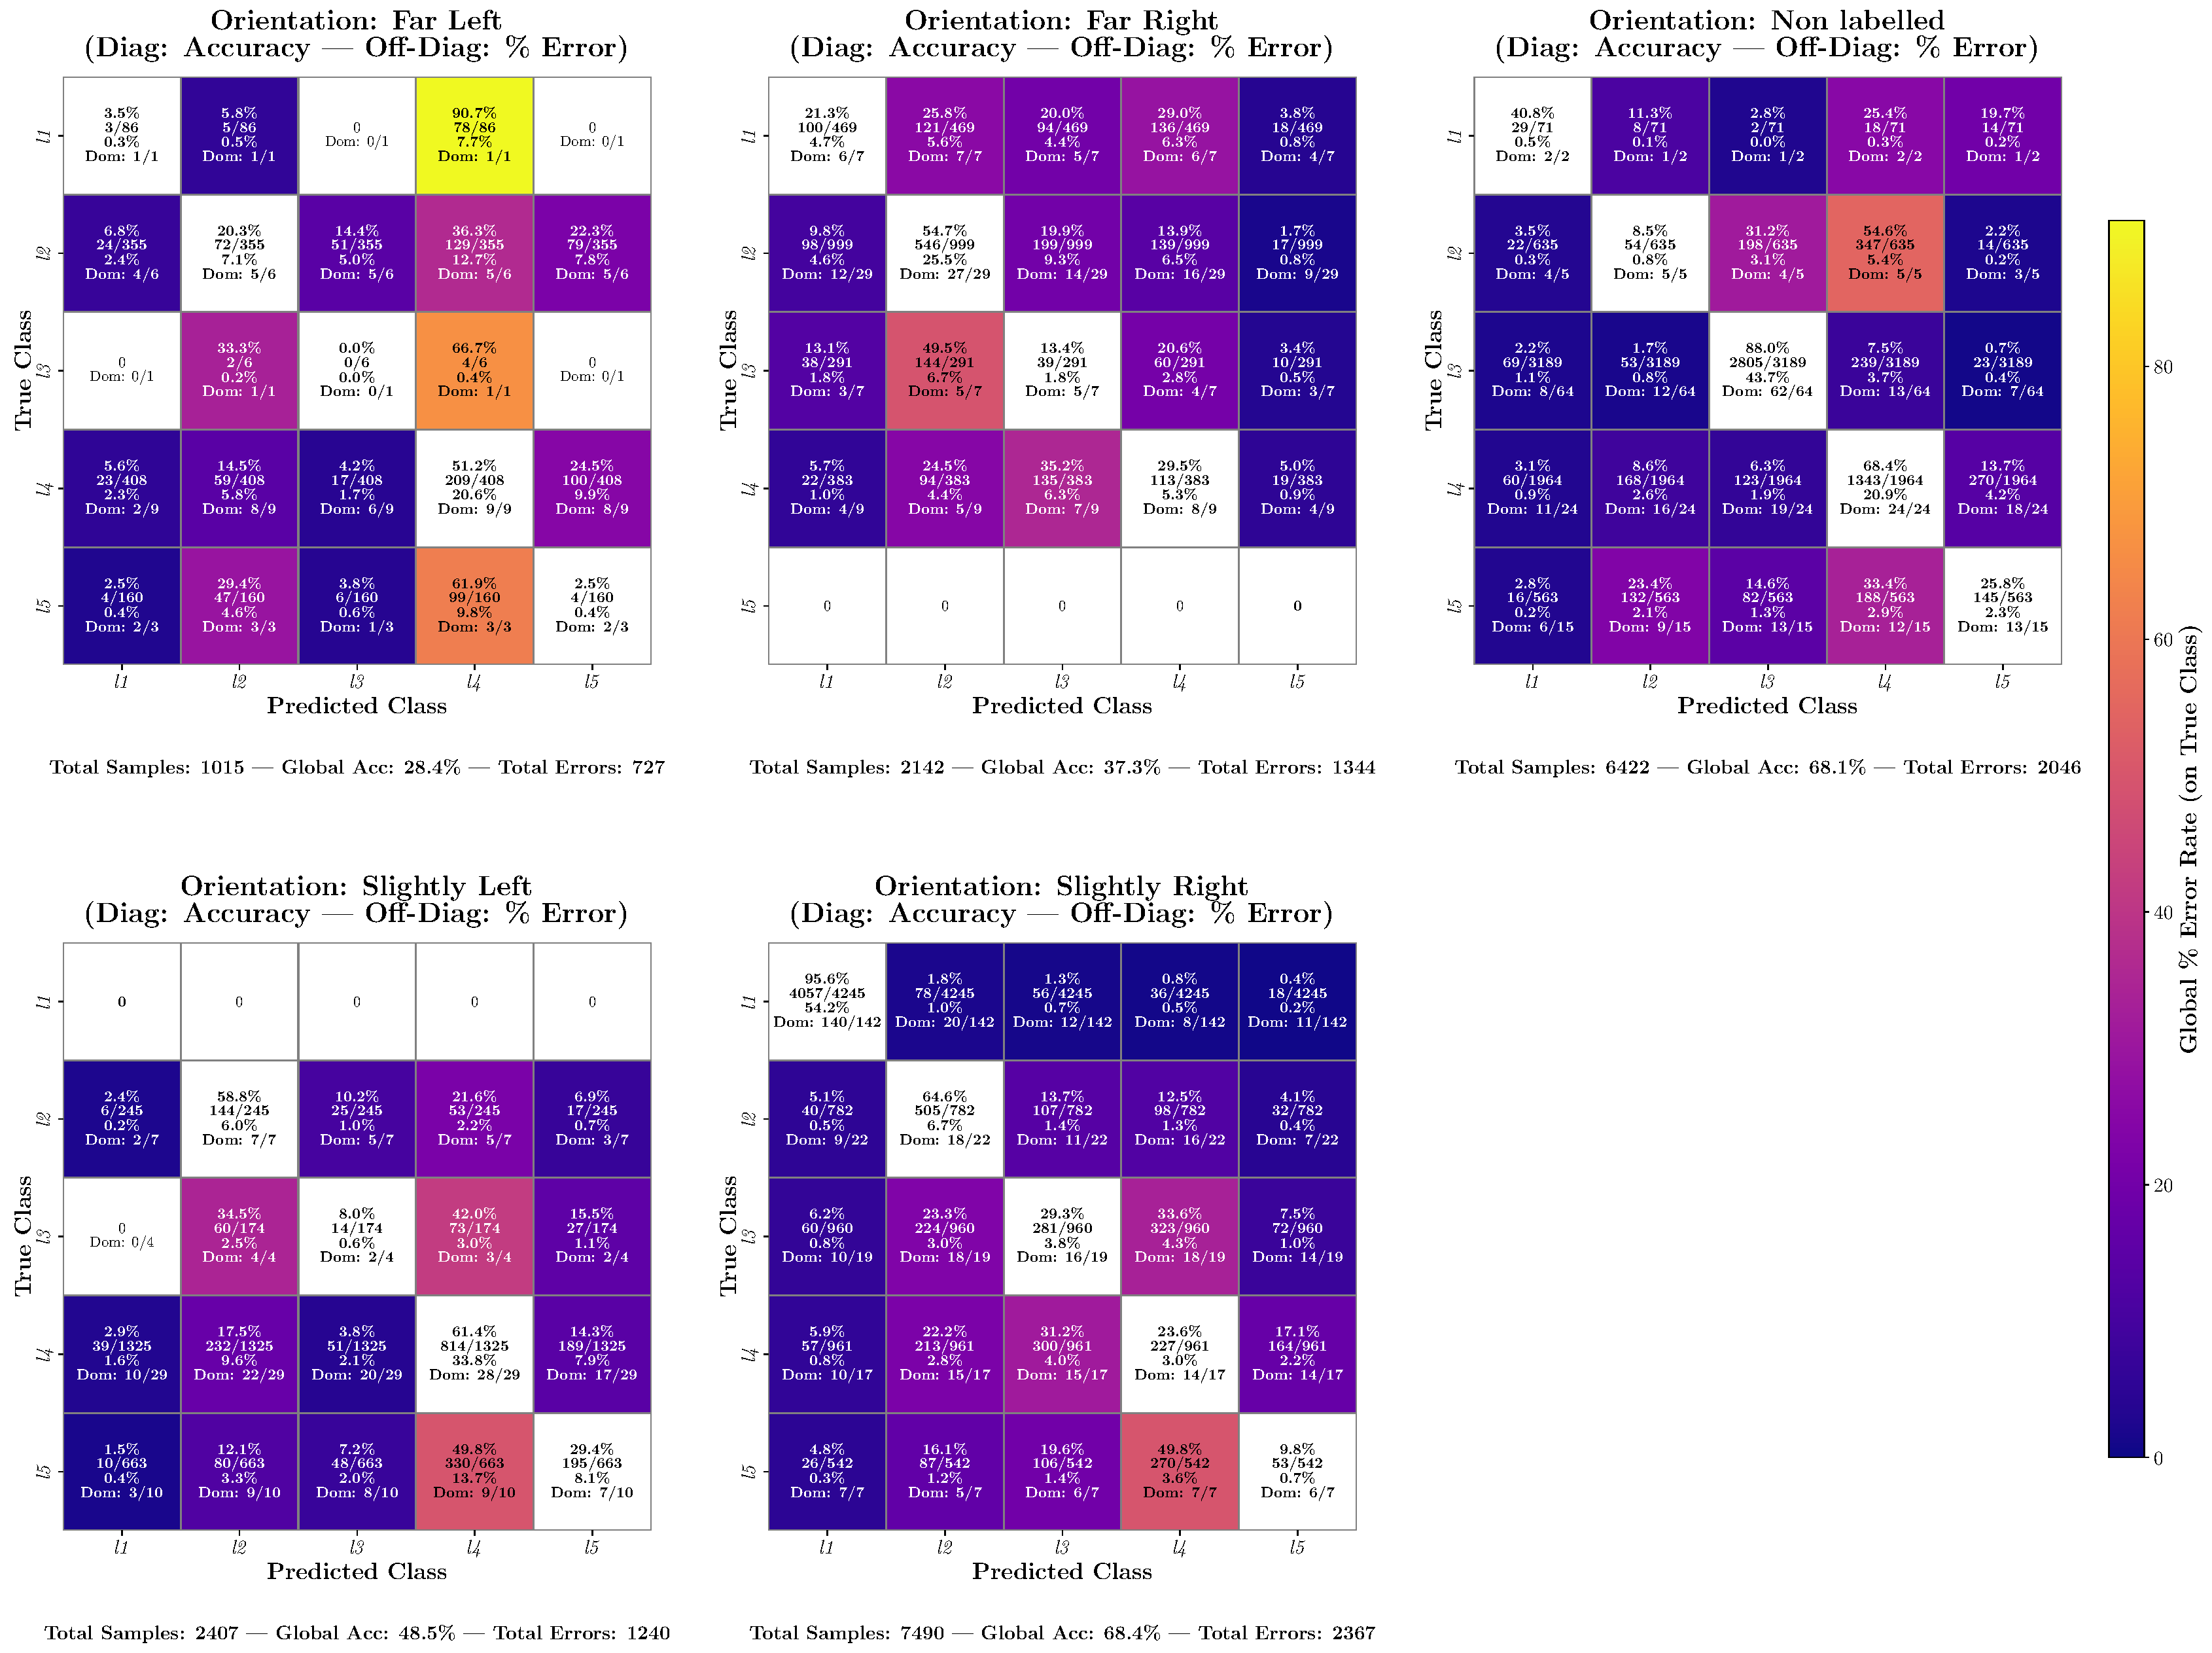
\includegraphics[width=\linewidth]{img/cmOnPoliticalLeaningRoberta.pdf}
  \caption{RoBERTa}
  \label{fig:cmPoliticalLeaningRoberta}
\end{subfigure}

\vspace{0.5cm}

% --- row 2 ---
\begin{subfigure}[b]{0.48\linewidth}
  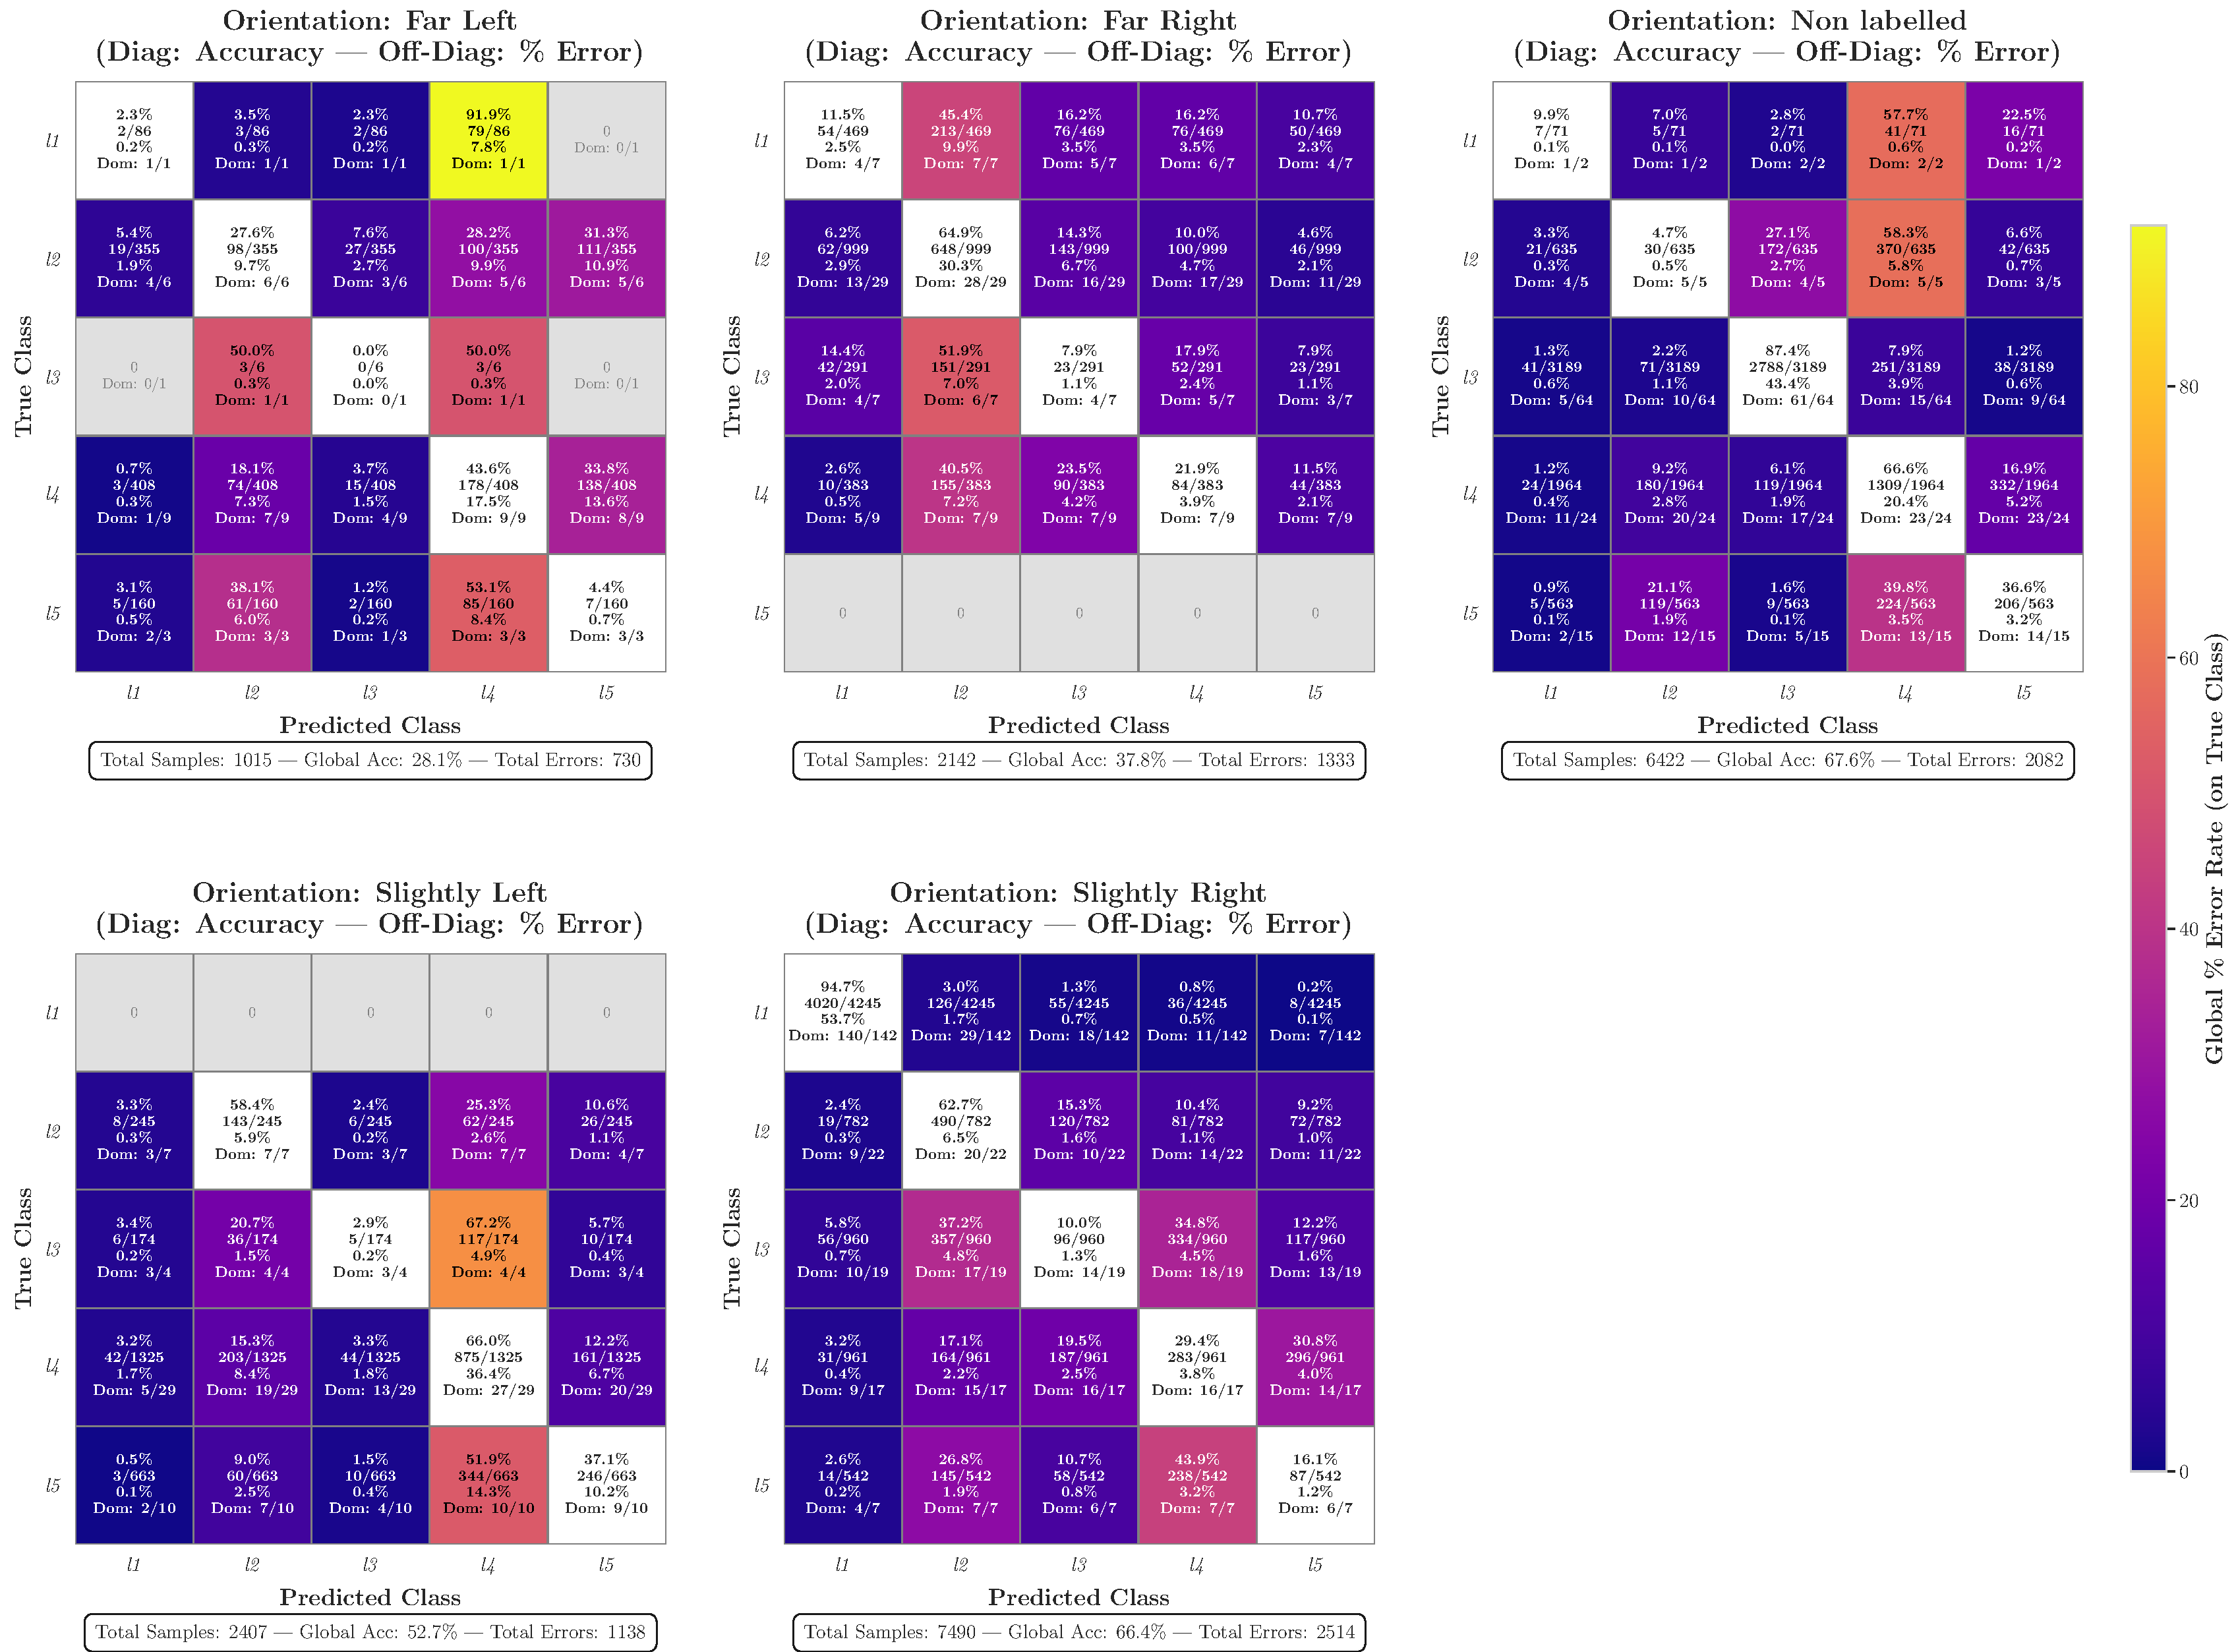
\includegraphics[width=\linewidth]{img/cmOnPoliticalLeaningLLama.pdf}
  \caption{Llama 3}
  \label{fig:cmPoliticalLeaningLlama}
\end{subfigure}\hfill
\begin{subfigure}[b]{0.48\linewidth}
  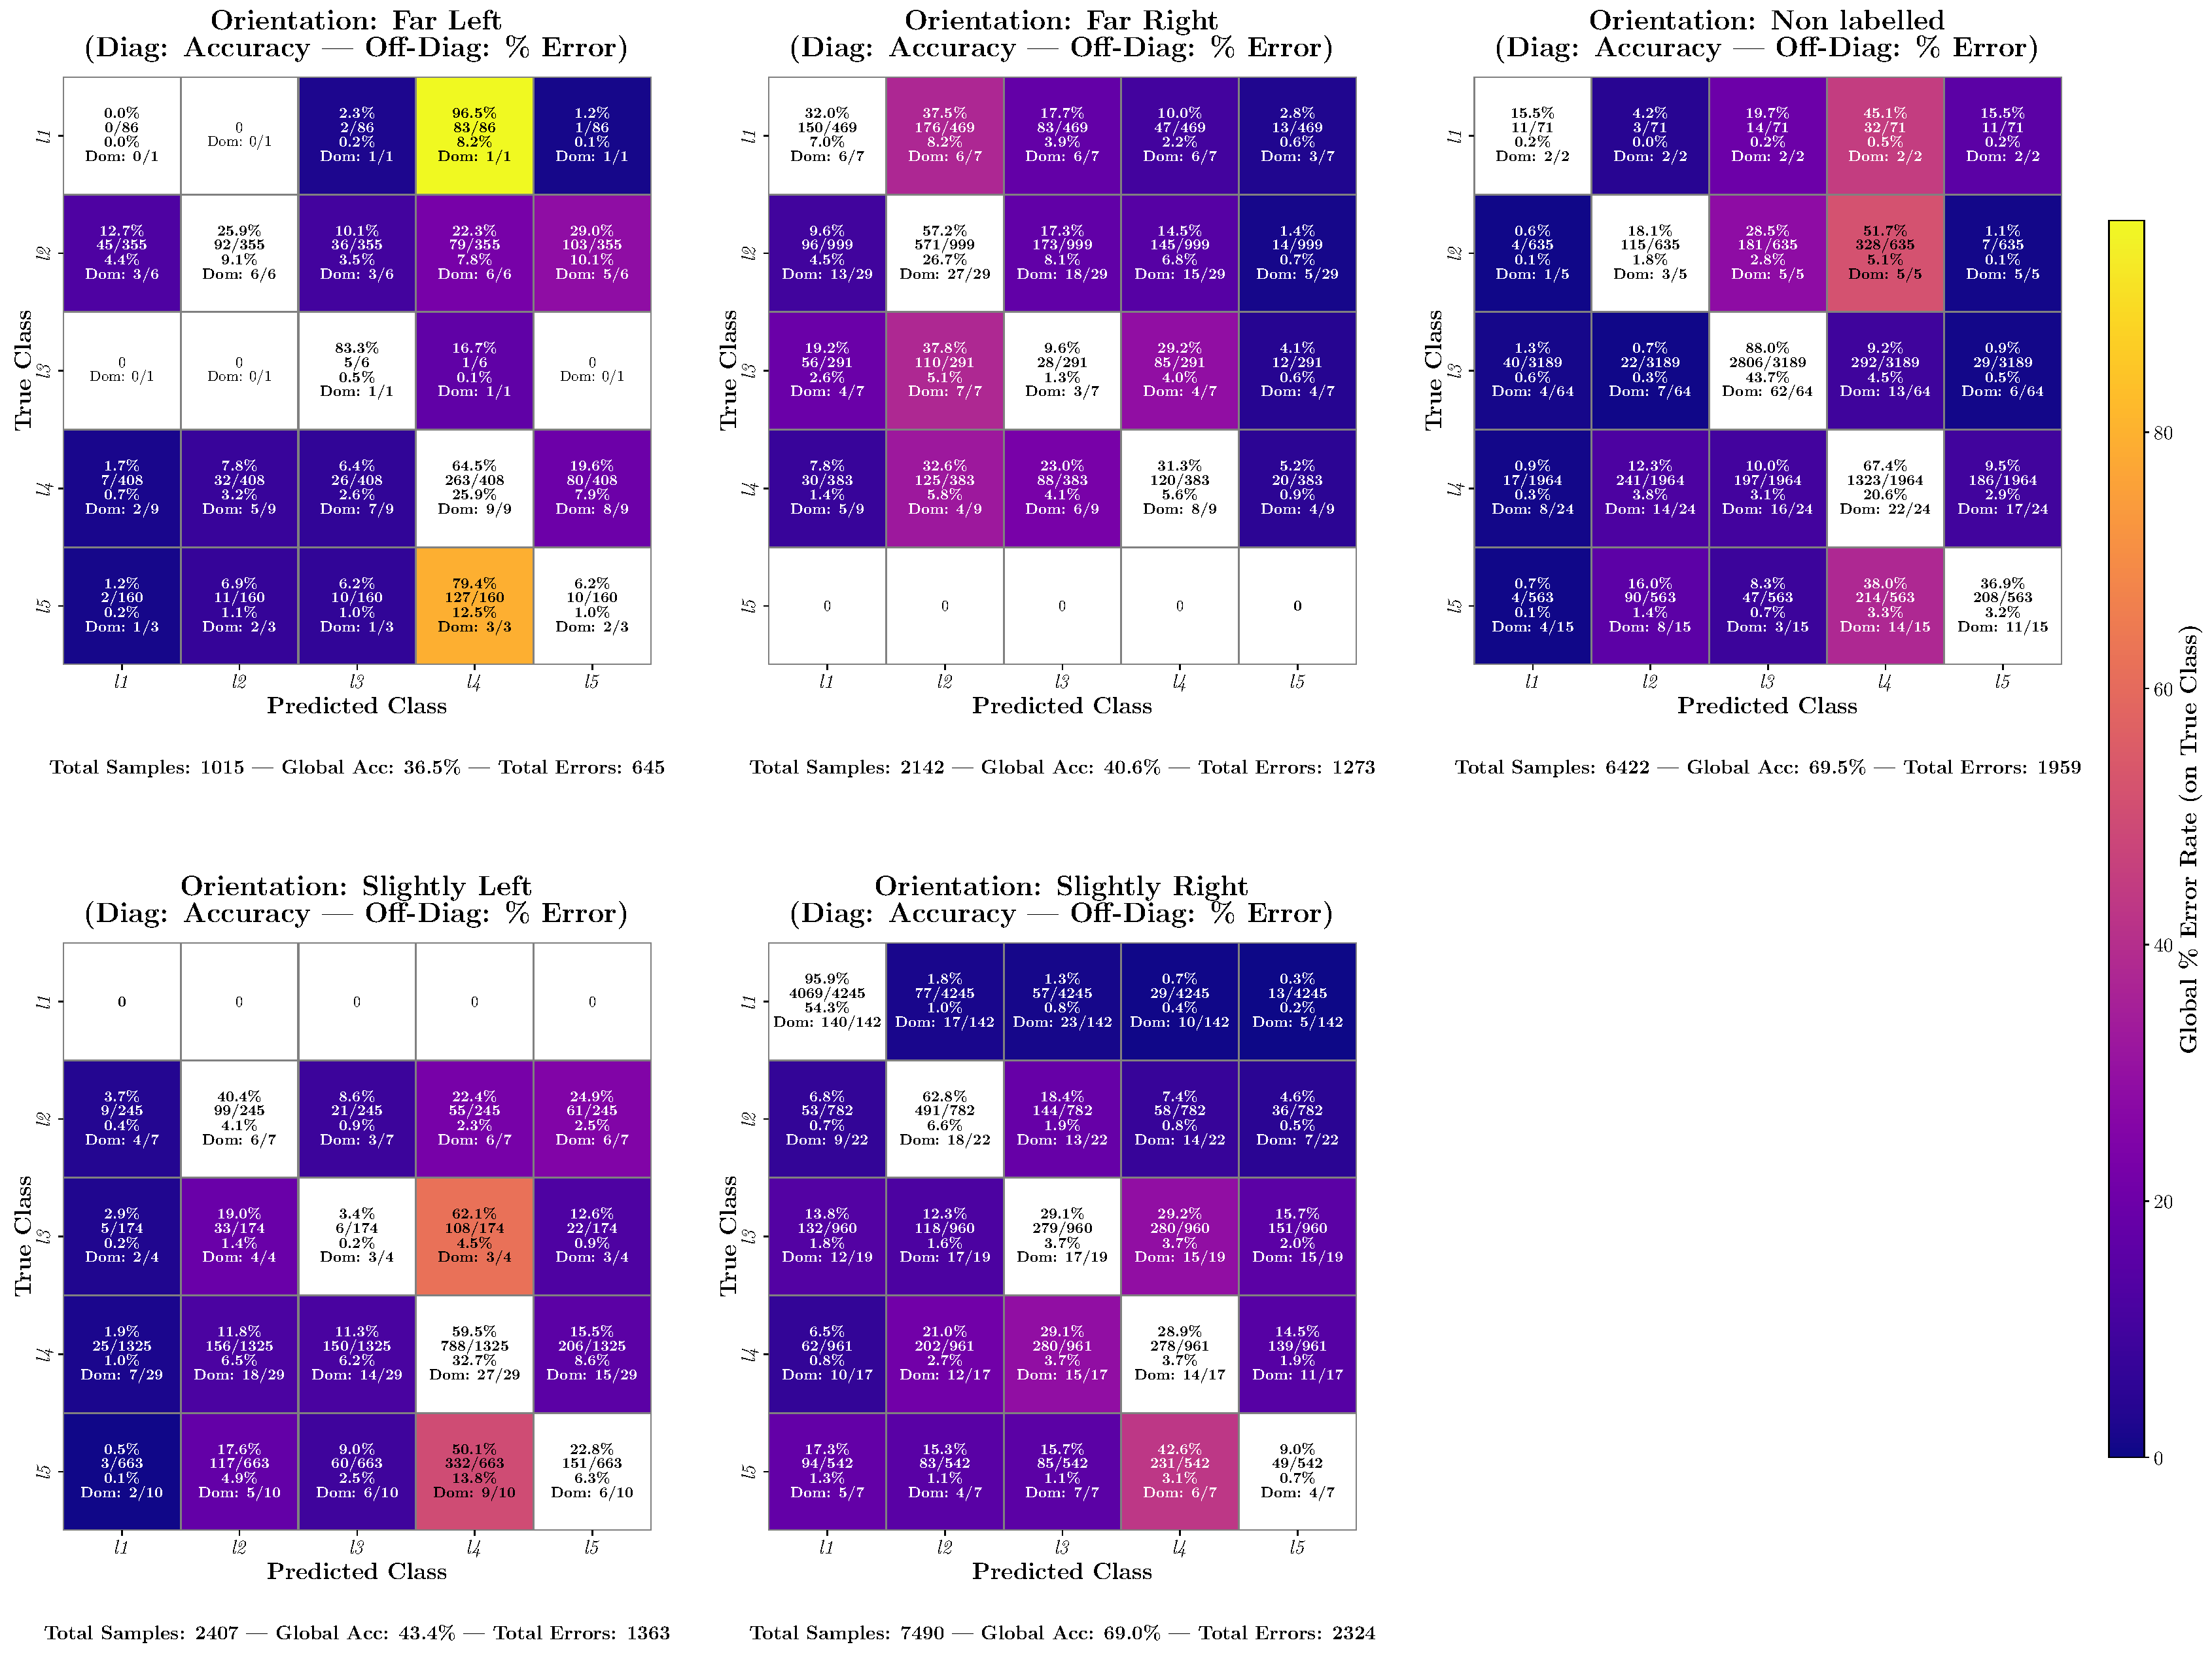
\includegraphics[width=\linewidth]{img/cmOnPoliticalLeaningMistral.pdf}
  \caption{Mistral}
  \label{fig:cmPoliticalLeaningMistral}
\end{subfigure}

\caption{Confusion matrices for political orientation across the four models. The rows correspond to the true labels and the columns to the predicted ones. The cells show class-wise percentages and counts, dataset-level percentages and contributing domains, and the colour represents the error rate per true class.}
\label{fig:cmPoliticalLeaning}
\end{figure*}


Figure \ref{fig:cmPoliticalLeaning} reveals why the Chi-square test rejects the hypothesis of independence: the distribution of errors varies between moderate and extreme political groups, with notable differences across models.
The matrices for `Slightly Right' and `Non-labelled' orientations exhibit strong diagonal dominance across all architectures. For the former (the largest group, $N=7490$), Mistral, RoBERTa, and BERT achieve comparable accuracies of 69.0\%, 68.4\%, and 67.6\%, respectively, with Llama 3 at 66.4\%. The domain counts (annotated as `Dom' in the cells) show that this performance is robust across a large number of unique sources.

In contrast, the `Far Left' ($N=1015$) and `Far Right' ($N=2142$) matrices display high off-diagonal scattering and significantly lower global accuracy.
For `Far Left', all models perform poorly with accuracies between 28.1\% and 29.5\% for the three smaller models and 36.5\% for Mistral.
Visual inspection confirms a systematic directional bias: predictions frequently land in the upper triangle of the matrix, confirming that models overestimate the reliability of these sources.

The `Far Right' category shows the greatest difference between the models. Mistral, Llama 3, and RoBERTa achieved 40.6\%, 37.8\%, and 37.3\%, respectively, while BERT dropped to 31.7\%.

Domain metrics further clarify that errors in these extreme categories are driven by a small set of outlets. Unlike the diverse `Slightly Right' group, the `Far Left' and `Far Right' categories contain fewer unique domains e.g., \textit{Dom: 1/1} or \textit{Dom: 5/7}, yet these specific outlets consistently trigger model errors.
The `Slightly Left' matrix confirms the specific discrediting pattern discussed in the main manuscript, where models tend to underestimate the reliability of slightly left-leaning sources.
A substantial cluster of misclassifications appears in the lower triangle, below the diagonal. This visually demonstrates that models penalize these articles, assigning them lower reliability labels compared to the ground truth, a behavior consistent across all four architectures.

We stress that these matrices are descriptive. Because political leaning and reliability are both properties of the publisher, and are themselves associated in the media ecosystem, the per-leaning error rates visible here cannot on their own separate a political effect from a reliability effect. The main paper addresses this with publisher-clustered tests that control for the true reliability level.


\section{Convergence Analysis}
\label{app:convergence}
To ascertain the most suitable training duration, a preliminary experiment involving 20 epochs was conducted using the Llama 3 model. As can be seen in Figure \ref{fig:loss_plot}, the model converges quickly. The validation loss reaches its minimum at epoch 4 (0.4416), after which the generalisation gap widens, indicating overfitting. The empirical evidence gathered from our most complex architecture validates our decision to limit fine-tuning to five epochs across all models, with the exception noted below.

We conducted an analogous convergence check for Mistral across the five-fold cross-validation. As can be seen in Figure \ref{fig:loss_mistral}, the training loss decreased sharply from an average of 2.02 at Epoch 1 to 0.36 at Epoch 2 and then to 0.23 at Epoch 3. The average improvement between epochs 2 and 3 is 0.13, indicating diminishing returns and stabilisation. This pattern mirrors the rapid convergence observed for Llama 3, supporting the idea of limiting Mistral training to three epochs to improve efficiency without compromising on convergence.


\begin{figure*}[!t]
\centering
\begin{subfigure}[b]{0.48\linewidth}
  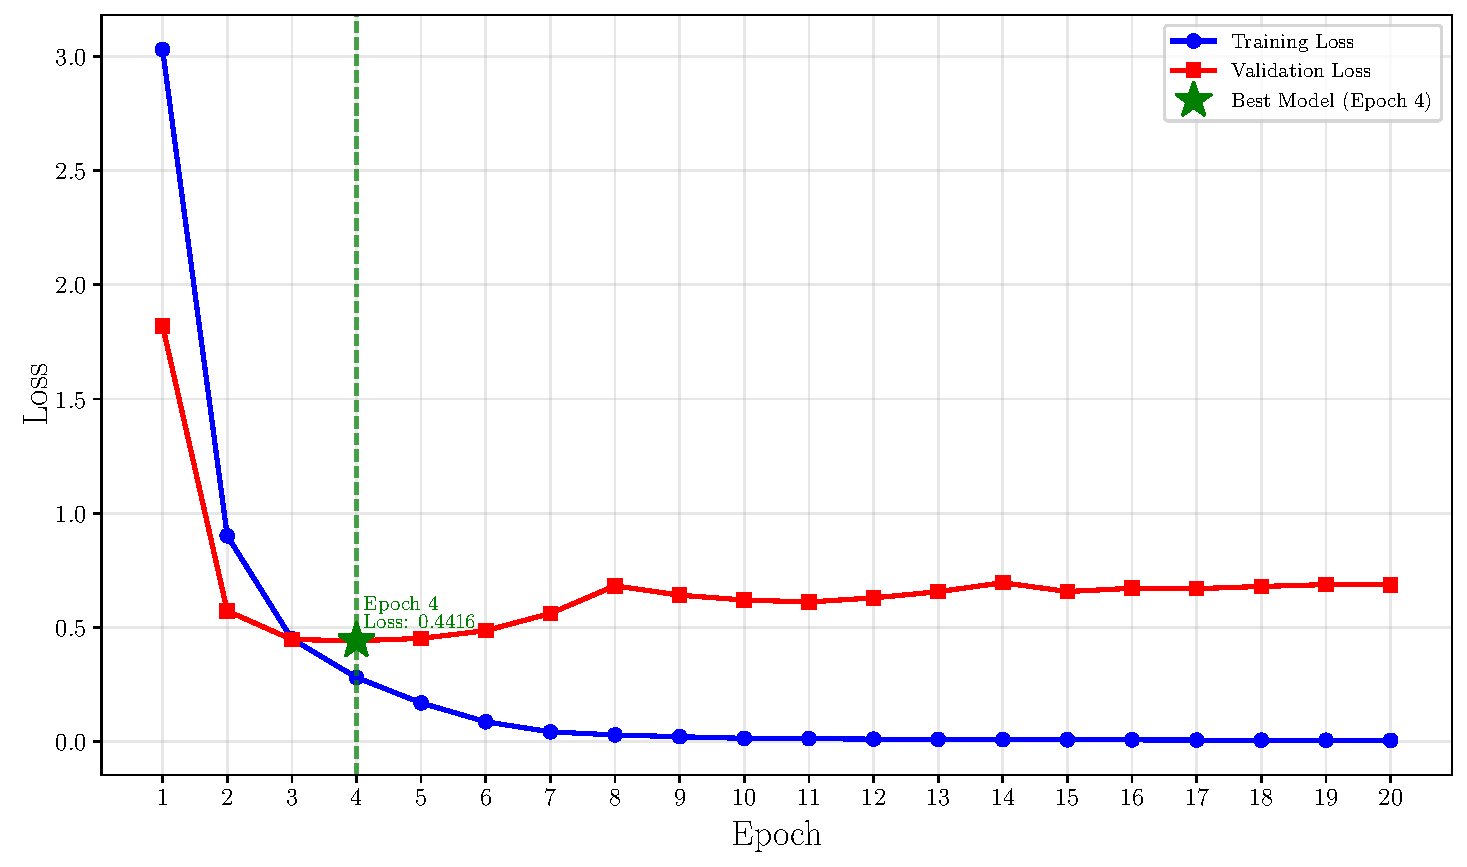
\includegraphics[width=\linewidth]{img/loss_plot.pdf}
  \caption{Training and Validation loss over 20 epochs for Llama 3. The green marker indicates the optimal model checkpoint at epoch 4. Longer training durations result in poorer generalisation performance.}
  \label{fig:loss_plot}
\end{subfigure}\hfill
\begin{subfigure}[b]{0.48\linewidth}
  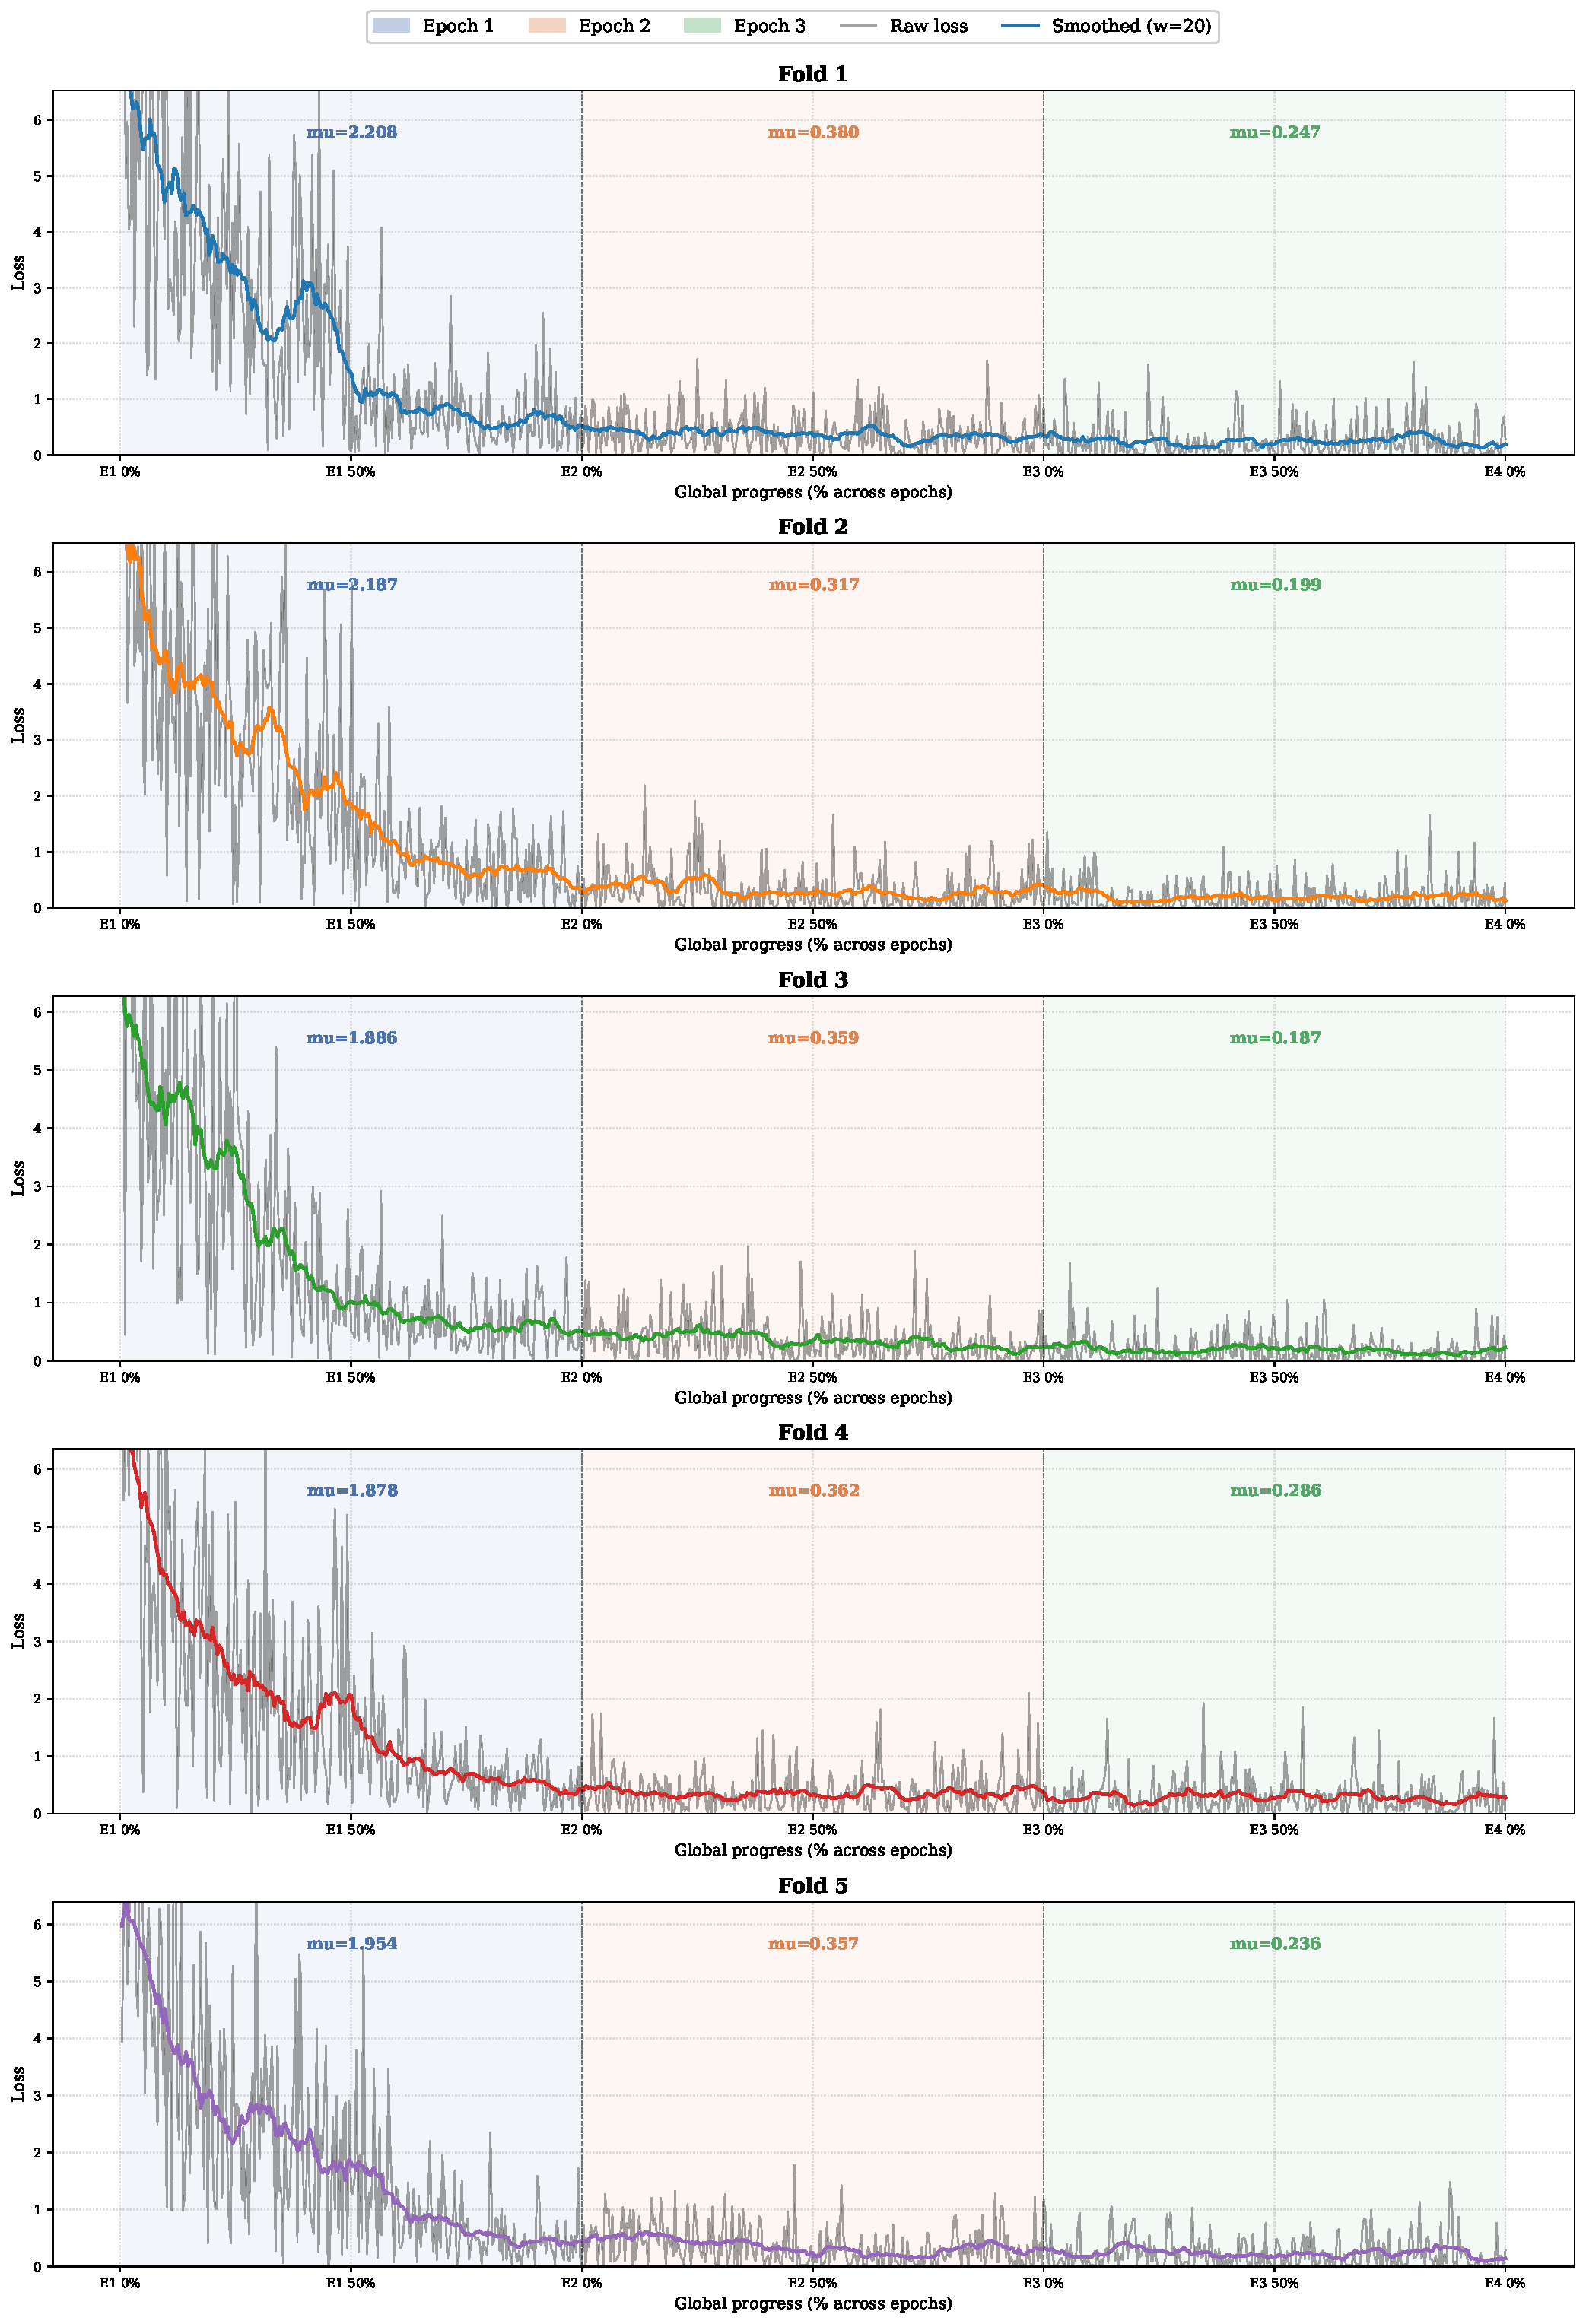
\includegraphics[width=\linewidth]{img/training_loss_mistral.pdf}
  \caption{Training loss over three epochs for Mistral, shown across five folds.}
  \label{fig:loss_mistral}
\end{subfigure}
\end{figure*}


\section{Reproducibility}
\label{app:repro}
Every figure in this document and in the main paper is regenerated from the
stored model predictions by a single notebook, so no figure depends on manual
steps or on the order in which cells were executed. The notebook also emits the
tables it reports, and validates that all four models are scored against the
same ground truth for the same article.


\bibliographystyle{plainnat}
\end{document}
